\section{Asymmetric Bidders}\label{sec:14-asym}

The models of \cref{sec:14-fpa,sec:14-mw-eq,sec:14-mw-rank} treat every bidder as a draw from the same
population, and the assessment in \cref{sec:14-mw-assessment} noted that symmetry is essential to the
Milgrom-Weber results. Many auctions instead pit different kinds of firms against each other. In the timber sales studied by
\citet{AtheyLevinSeira2011}, sawmills with their own manufacturing capacity compete with independent
loggers who must resell the timber. In public procurement, domestic firms compete with foreign firms,
and incumbents compete with entrants. This section develops the private values model with bidders
who draw their values from different distributions.

The mechanism-design results of \cref{sec:14-ret} already allow bidder-specific distributions.
Revenue equivalence therefore still holds for any two auctions that allocate the object in the same
way. Asymmetry matters because it makes the first-price auction allocate the object differently from
the second-price and ascending auctions. We show how the allocation changes, who gains and who loses,
and why the revenue comparison becomes ambiguous.

\subsection{The asymmetric private values model}\label{sec:14-asym-model}

\begin{assumption}[Asymmetric independent private values]\label{ass:14-asym}
There are $n\ge 2$ risk-neutral bidders, $i\in\mathcal N=\{1,\dots,n\}$. Bidder $i$'s value $V_i$ is
drawn from a distribution $F_i$ with a continuous density $f_i$ that is strictly positive on the
support $[\underline v,\bar v_i]$. Values are independent across bidders and private. The
distributions $F_1,\dots,F_n$ and the set of bidders are common knowledge. The reserve price equals
the common lower bound of the supports, $r=\underline v$.
\end{assumption}

The common lower bound and the choice $r=\underline v$ follow the model of
\citet[Section II.A]{AtheyLevinSeira2011}, where every support has the form $[\underline v=r,\bar
v_i]$. The upper bounds may differ. When there are two classes of bidders, we call them
\emph{strong} (subscript $s$) and \emph{weak} (subscript $w$). The ordering that gives these labels
content is the following.

\begin{definition}[Stochastic orders]\label{def:14-rhr}
Let $F_s$ and $F_w$ have the common lower bound $\underline v$, and set $f_i(v)=0$ and $F_i(v)=1$
for $v>\bar v_i$. The distribution $F_s$ dominates $F_w$ in the \emph{reverse hazard rate order} if
\begin{equation}\label{eq:14-rhr}
\frac{f_s(v)}{F_s(v)}\;\ge\;\frac{f_w(v)}{F_w(v)}\qquad\text{for all } v>\underline v .
\end{equation}
It dominates in the \emph{hazard rate order} if $\frac{f_s(v)}{1-F_s(v)}\le\frac{f_w(v)}{1-F_w(v)}$
wherever both ratios are defined. It dominates in the \emph{likelihood ratio order} if
$\frac{f_s(v)}{f_w(v)}$ is nondecreasing. It dominates in the sense of \emph{first-order stochastic
dominance} if $F_s(v)\le F_w(v)$ for all $v$.
\end{definition}

The ratio $\frac{f(v)}{F(v)}$ is the \emph{reverse hazard rate}. It is the density of the value at
$v$ conditional on the value not exceeding $v$. Condition \eqref{eq:14-rhr} says that, conditional on
both values lying below any level $v$, the strong value is more concentrated near the top. Since
$\frac{f}{F}=\frac{d}{dv}\ln F$, condition \eqref{eq:14-rhr} is equivalent to
\begin{equation}\label{eq:14-rhr-ratio}
\frac{d}{dv}\ln\frac{F_s(v)}{F_w(v)}\ge 0,\qquad\text{so that } \frac{F_s(v)}{F_w(v)}\text{ is nondecreasing in } v .
\end{equation}
The likelihood ratio order implies both the reverse hazard rate order and the hazard rate order, and
each of these implies first-order dominance \citep[see][]{Krishna2010}. \Cref{prop:B-orders-chain}
proves this chain, and \cref{sec:B-stochastic-orders} restates the four orders for reference. The reverse hazard rate
order is the one that signs equilibrium bids in the first-price auction
\citep{MaskinRiley2000,AtheyLevinSeira2011}. A reader of the original papers should note one difference in
names. \citet[Section~II.A, p.~212]{AtheyLevinSeira2011} assume that $F_M$ dominates $F_L$ ``according to a
hazard rate order,'' with mills $M$ strong and loggers $L$ weak. Their condition is
$\frac{f_M(v)}{F_M(v)}\ge\frac{f_L(v)}{F_L(v)}$, which is the reverse hazard rate order \eqref{eq:14-rhr} of
our definition.

\begin{lemma}\label{lem:14-rhr-fosd}
If $F_s$ dominates $F_w$ in the reverse hazard rate order, then $\bar v_s\ge\bar v_w$ and
$F_s(v)\le F_w(v)$ for all $v$. Strong values first-order stochastically dominate weak values.
\end{lemma}

\begin{proof}
Suppose first that $\bar v_s<\bar v_w$. For $v\in(\bar v_s,\bar v_w)$ the left side of
\eqref{eq:14-rhr} is zero, because $f_s(v)=0$, while the right side is strictly positive. This
contradicts \eqref{eq:14-rhr}, so $\bar v_s\ge\bar v_w$.

By \eqref{eq:14-rhr-ratio}, the ratio $\frac{F_s}{F_w}$ is nondecreasing on $(\underline v,\bar v_s]$.
At $v=\bar v_s$ both distributions equal one, because $\bar v_s\ge\bar v_w$. Hence, for every
$v\in(\underline v,\bar v_s]$,
\[
\frac{F_s(v)}{F_w(v)}\le\frac{F_s(\bar v_s)}{F_w(\bar v_s)}=1 .
\]
Multiplying by $F_w(v)>0$ gives $F_s(v)\le F_w(v)$. Above $\bar v_s$ both distributions equal one.
\end{proof}

Two examples recur below. First, let $F_i$ be uniform on $[0,\bar v_i]$ with $\bar v_s>\bar v_w$.
Then $\frac{f_i(v)}{F_i(v)}=\frac{1}{v}$ for both bidders on $(0,\bar v_w]$. Above $\bar v_w$ the weak
bidder's reverse hazard rate is zero and the strong bidder's is $\frac{1}{v}$. Condition
\eqref{eq:14-rhr} holds, with equality on the common part of the supports. Second, let
$F_i(v)=\left(\frac{v}{\bar v}\right)^{\gamma_i}$ on a common support $[0,\bar v]$. The reverse hazard
rate is $\frac{\gamma_i}{v}$, so $F_s$ dominates $F_w$ exactly when $\gamma_s\ge\gamma_w$.

\subsection{Second-price and ascending auctions with asymmetric bidders}\label{sec:14-asym-spa}

Asymmetry leaves the second-price and ascending auctions unchanged in their essentials. The dominance
argument of \cref{prop:14-spa-dominant} uses only private values. Each bidder therefore still bids its
value in the second-price auction and stays in the button auction until the price reaches its value
\citep[Section II.B]{AtheyLevinSeira2011}. The highest-value bidder wins, so both auctions are
\emph{efficient}. The price is the second-highest value, because $r=\underline v$.

The distribution of the price follows from counting. Let $V^{(2)}$ denote the second-highest of the $n$
values. It is at most $t$ when
all values are at most $t$, or when exactly one value exceeds $t$:
\begin{equation}\label{eq:14-asym-second}
\Pr\left(V^{(2)}\le t\right)=\prod_{j=1}^{n}F_j(t)+\sum_{i=1}^{n}\bigl(1-F_i(t)\bigr)\prod_{j\neq i}F_j(t).
\end{equation}
Expected revenue is $R^{SP}=\underline v+\int_{\underline v}^{\bar v}\bigl[1-\Pr(V^{(2)}\le
t)\bigr]dt$ with $\bar v=\max_i\bar v_i$. Bidder $i$ of type $v$ wins with probability
$Q_i^{SP}(v)=\prod_{j\neq i}F_j(v)$. The lowest type earns zero, so \cref{lem:14-ic} gives its
interim expected surplus,
\begin{equation}\label{eq:14-asym-spa-payoff}
\pi_i^{SP}(v)=\int_{\underline v}^{v}\prod_{j\neq i}F_j(t)\,dt .
\end{equation}

\subsection{The first-price auction: first-order conditions}\label{sec:14-asym-foc}

Suppose every rival $j$ uses a strictly increasing, differentiable bid function $\beta_j$ with inverse
$\phi_j=\beta_j^{-1}$. Rival $j$ bids less than $b$ with probability
\begin{equation}\label{eq:14-asym-G}
G_j(b)=\Pr\bigl(\beta_j(V_j)<b\bigr)=F_j\bigl(\phi_j(b)\bigr),
\end{equation}
which is \citet[eq. (1)]{AtheyLevinSeira2011}. Let $g_j=G_j'$ be the density of $j$'s bid. Bid
distributions are continuous, so ties occur with probability zero. Bidder $i$ with value $v_i$ wins
with bid $b$ when every rival bids less, and independence gives the expected payoff
\begin{equation}\label{eq:14-asym-payoff}
U_i(b;v_i)=(v_i-b)\prod_{j\neq i}G_j(b).
\end{equation}
The payoff is the product of a margin and a win probability. Taking logarithms turns the product into
a sum,
\[
\ln U_i(b;v_i)=\ln(v_i-b)+\sum_{j\neq i}\ln G_j(b).
\]
Differentiating with respect to $b$ and setting the derivative to zero at the optimal bid $b_i$ gives
\[
-\frac{1}{v_i-b_i}+\sum_{j\neq i}\frac{g_j(b_i)}{G_j(b_i)}=0 .
\]
Rearranging yields the first-order condition of the asymmetric first-price auction:
\begin{equation}\label{eq:14-asym-foc}
\frac{1}{v_i-b_i}=\sum_{j\neq i}\frac{g_j(b_i)}{G_j(b_i)} .
\end{equation}
This is \citet[eq. (2)]{AtheyLevinSeira2011}. The left side is the proportional loss in the margin
from raising the bid. The right side is the proportional gain in the win probability, summed over the
rivals who might be outbid. Solving \eqref{eq:14-asym-foc} for the value gives the inverse form
\begin{equation}\label{eq:14-asym-inverse}
v_i=b_i+\left[\sum_{j\neq i}\frac{g_j(b_i)}{G_j(b_i)}\right]^{-1}.
\end{equation}
Equation \eqref{eq:14-asym-inverse} expresses each bidder's value through its own bid and the
distributions of its rivals' bids. With $n-1$ identical rivals the sum equals $(n-1)\frac{g}{G}$, and
\eqref{eq:14-asym-inverse} reduces to the symmetric condition \eqref{eq:14-foc-G}. \Cref{ch:auction-empirics} uses \eqref{eq:14-asym-inverse} to recover asymmetric value distributions
from bids.

\casehead{The system of differential equations}
The first-order conditions hold for every bidder at every bid, so they jointly determine the inverse
bid functions. Write $\nu_j(b)=\frac{g_j(b)}{G_j(b)}$ for the reverse hazard rate of $j$'s bid and
$\bar\nu(b)=\sum_{j=1}^{n}\nu_j(b)$ for their sum. Here $\nu$ is unrelated to the taste shocks of
the demand chapters. At bid $b$, bidder $i$'s value is $\phi_i(b)$, so
\eqref{eq:14-asym-foc} reads
\begin{equation}\label{eq:14-asym-foc-lambda}
\bar\nu(b)-\nu_i(b)=\frac{1}{\phi_i(b)-b},\qquad i=1,\dots,n .
\end{equation}
Summing \eqref{eq:14-asym-foc-lambda} over the $n$ bidders gives
$n\bar\nu(b)-\bar\nu(b)=\sum_{j}\frac{1}{\phi_j(b)-b}$, and therefore
\[
\bar\nu(b)=\frac{1}{n-1}\sum_{j=1}^{n}\frac{1}{\phi_j(b)-b}.
\]
Substituting back into \eqref{eq:14-asym-foc-lambda} isolates each bidder's own term:
\[
\nu_i(b)=\frac{1}{n-1}\sum_{j=1}^{n}\frac{1}{\phi_j(b)-b}-\frac{1}{\phi_i(b)-b}.
\]
By \eqref{eq:14-asym-G}, $\nu_i(b)=\frac{f_i(\phi_i(b))\,\phi_i'(b)}{F_i(\phi_i(b))}$. Solving for
$\phi_i'(b)$ gives the system
\begin{equation}\label{eq:14-asym-ode}
\phi_i'(b)=\frac{F_i\bigl(\phi_i(b)\bigr)}{f_i\bigl(\phi_i(b)\bigr)}
\left[\frac{1}{n-1}\sum_{j=1}^{n}\frac{1}{\phi_j(b)-b}-\frac{1}{\phi_i(b)-b}\right],\qquad i=1,\dots,n.
\end{equation}
With two bidders the bracket equals $\frac{1}{\phi_1-b}+\frac{1}{\phi_2-b}-\frac{1}{\phi_i-b}$, so
the system collapses to
\begin{equation}\label{eq:14-asym-ode2}
\phi_i'(b)=\frac{F_i\bigl(\phi_i(b)\bigr)}{f_i\bigl(\phi_i(b)\bigr)}\,\frac{1}{\phi_j(b)-b},\qquad
i,j\in\{1,2\},\ j\neq i .
\end{equation}
Each bidder's inverse bid function depends on its rival's through the rival's margin
$\phi_j(b)-b$. An equivalent form, used repeatedly below, is
\begin{equation}\label{eq:14-asym-logG}
\frac{d}{db}\ln G_j(b)=\frac{1}{\phi_i(b)-b}\qquad\text{(two bidders, } j\neq i\text{)} .
\end{equation}

The system needs boundary conditions. At the bottom, every bidder bids the reserve price,
$\phi_i(r)=r$ for all $i$ \citep[Section II.B]{AtheyLevinSeira2011}. At the top, each bidder's
highest type submits that bidder's highest bid $\bar b_i$, so $\phi_i(\bar b_i)=\bar v_i$. The top
bids coincide in two cases covered by \cref{prop:14-common-support} below. The first is two
bidders, with any upper bounds $\bar v_1$ and $\bar v_2$. The second is any number of bidders whose
values share one support. In either case all bidders have a common top bid $\bar b$, and
$\phi_i(\bar b)=\bar v_i$ for every $i$. With three or more bidders and different upper bounds, the
top bids can differ (see the remark after the proposition). Bidder $i$ then leaves the system
\eqref{eq:14-asym-ode} above $\bar b_i$, and each endpoint $\bar b_i$ must be found as part of the
solution. In the two cases with a common top bid, $\bar b$ is itself unknown. The problem is
therefore a two-point boundary value problem with a free endpoint. The right side of
\eqref{eq:14-asym-ode} is singular at $b=r$, where every margin $\phi_j(b)-b$ vanishes. Numerical
methods therefore guess $\bar b$, integrate backward from the top and adjust the guess until every
$\phi_i$ reaches $r$ at $b=r$ \citep{MarshallEtAl1994,Bajari2001}.

\casehead{Type-symmetric bidding}
In the application of \citet{AtheyLevinSeira2011} the participants consist of $n_L$ weak bidders
(loggers) and $n_M$ strong bidders (mills), with $\bm n=(n_L,n_M)$ and $n=n_L+n_M$. Bidders of the
same type use the same bid function. We write $G_L(\cdot;\bm n)$ and $G_M(\cdot;\bm n)$ for the bid
distributions of one logger and one mill, and $\phi_L$ and $\phi_M$ for the inverse bid functions. A logger
faces $n_L-1$ other loggers and $n_M$ mills, and a mill faces $n_L$ loggers and $n_M-1$ other mills.
Condition \eqref{eq:14-asym-foc} becomes
\begin{align}
\frac{1}{\phi_L(b)-b}&=(n_L-1)\frac{g_L(b;\bm n)}{G_L(b;\bm n)}+n_M\frac{g_M(b;\bm n)}{G_M(b;\bm n)},\label{eq:14-ts-foc-L}\\
\frac{1}{\phi_M(b)-b}&=n_L\frac{g_L(b;\bm n)}{G_L(b;\bm n)}+(n_M-1)\frac{g_M(b;\bm n)}{G_M(b;\bm n)}.\label{eq:14-ts-foc-M}
\end{align}
Applying the solution of \eqref{eq:14-asym-foc-lambda} with $n_L$ copies of $\phi_L$ and $n_M$
copies of $\phi_M$ gives, for $k\in\{L,M\}$,
\begin{equation}\label{eq:14-ts-lambda}
\frac{g_k(b;\bm n)}{G_k(b;\bm n)}=\frac{1}{n-1}\left[\frac{n_L}{\phi_L(b)-b}+\frac{n_M}{\phi_M(b)-b}\right]-\frac{1}{\phi_k(b)-b}.
\end{equation}
When $\phi_L=\phi_M=\phi$, the right side equals $\frac{1}{(n-1)(\phi(b)-b)}$. This recovers the
symmetric condition $v=b+\frac{G(b)}{(n-1)g(b)}$, as it should.

\subsection{Common support of the bid distributions*}\label{sec:14-asym-support}

The boundary condition at the top rests on the following result.

\begin{proposition}[Common bid support]\label{prop:14-common-support}
Consider an equilibrium of the first-price auction in strictly increasing bid functions under
\cref{ass:14-asym}. Let $\bar b_i$ be the highest bid of bidder $i$.
\begin{enumerate}[label=(\alph*)]
\item With two bidders, $\bar b_1=\bar b_2$, whether or not the value supports coincide.
\item \citep[Theorem 2.2]{AtheyHaile2007} With $n\ge 2$ bidders whose values share the support
$[\underline v,\bar v]$, all bidders have the same bid support $[r,\bar b]$.
\end{enumerate}
\end{proposition}

\begin{proof}
(a) Suppose $\bar b_j>\bar b_i$. Every bid $b\in(\bar b_i,\bar b_j]$ wins against bidder $i$ with
probability one. A type of bidder $j$ that bids such a $b$ could lower its bid to any level in
$(\bar b_i,b)$, still win with probability one and pay less. So no type of $j$ bids above $\bar
b_i$, which contradicts $\bar b_j>\bar b_i$.

(b) We follow \citet[proof of Theorem 2.2]{AtheyHaile2007}. With independence, the inverse bid
function of bidder $i$ is the right side of \eqref{eq:14-asym-inverse},
\[
\xi_i(b)=b+\left[\sum_{k\neq i}\frac{g_k(b)}{G_k(b)}\right]^{-1}.
\]
Part (a) covers $n=2$, so let $n>2$ and suppose $\bar b_i<\bar b_j$. The highest type $\bar v$ of
bidder $i$ bids $\bar b_i$, so
\[
\bar v=\xi_i(\bar b_i)=\bar b_i+\left[\sum_{k\in\mathcal N\setminus\{i\}}\frac{g_k(\bar b_i)}{G_k(\bar
b_i)}\right]^{-1}.
\]
Bidder $j$'s inverse bid function must be continuous at $\bar b_i$. Otherwise a strictly increasing
strategy would leave a gap in $j$'s values, which contradicts an interval support. Just above $\bar
b_i$ bidder $i$ never bids, so $G_i=1$ and $g_i=0$ there, and bidder $i$ drops out of $j$'s sum. The
remaining sum omits the strictly positive term $\frac{g_j(\bar b_i)}{G_j(\bar b_i)}$ that appears in
bidder $i$'s sum. Hence
\[
\bar v=\xi_i(\bar b_i)<\bar b_i+\left[\sum_{k\in\mathcal N\setminus\{i,j\}}\frac{g_k(\bar
b_i)}{G_k(\bar b_i)}\right]^{-1}=\xi_j(\bar b_i).
\]
So bidder $j$'s type that bids $\bar b_i$ has a value above $\bar v$, which contradicts the common
support. All highest bids are therefore equal. Standard arguments show that every bid support starts
at $r$, which gives the common support $[r,\bar b]$.
\end{proof}

Part (b) needs the common value support when $n>2$. \citet[footnote 15]{AtheyHaile2007} give a
three-bidder example with different value supports in which the bid supports differ. With two
bidders, part (a) shows that the top bid is common even when $\bar v_s>\bar v_w$, as in the uniform
example below. The type-symmetric model of \cref{sec:14-asym-foc} falls outside both parts when it
has more than two participants and the two types have different upper bounds. A common top bid then
cannot be imposed without further argument.

\casehead{Existence and uniqueness}
\citet[Theorem~2.1]{AtheyHaile2007} summarize the results for first-price auctions in which values
have a compact, convex support and signals are affiliated with a positive density. An equilibrium in
pure, nondecreasing strategies exists, by \citet{Athey2001} and \citet{RenyZamir2004}
\citep[footnote~10]{AtheyHaile2007}. An equilibrium in strictly increasing strategies exists in every
such model except common values with asymmetric bidders and dependent signals. With independent
private values and a continuously differentiable density, the equilibrium is unique, and it is in
pure, strictly increasing and differentiable strategies \citep[Theorem~2.1(ii)]{AtheyHaile2007}. In
that case all equilibria are monotone. The uniqueness results are due to \citet{Lebrun1999},
\citet{Bajari2001} and \citet{MaskinRiley2003} \citep[footnote~11]{AtheyHaile2007}. \citet{Lebrun1999}
also gives an alternative proof of the common bid support of \cref{prop:14-common-support}
\citep[footnote~14]{AtheyHaile2007}. \citet{Lebrun1996} had earlier proved existence in strictly
increasing bid functions for asymmetric independent private values.
The first-order conditions and the boundary condition $\phi_i(r)=r$ then characterize the equilibrium
bids for any set of participants \citep[Section II.B]{AtheyLevinSeira2011}.

\subsection{Strong bidders shade more: the Maskin-Riley properties}\label{sec:14-asym-mr}

The main qualitative results compare the two classes of bidders. They hold under the reverse hazard
rate order and are due to \citet{MaskinRiley2000}. We state and prove them for two bidders.
\citet[Section II.B]{AtheyLevinSeira2011} state properties (i) and (ii) for type-symmetric
equilibria with any numbers of mills and loggers.

\begin{proposition}[Maskin and Riley 2000]\label{prop:14-maskin-riley}
Let there be one strong and one weak bidder satisfying \cref{ass:14-asym}, with $F_s$ dominating $F_w$
in the reverse hazard rate order. In the equilibrium of the first-price auction with strictly
increasing bid functions:
\begin{enumerate}[label=(\roman*)]
\item The strong bidder shades more. At every bid the strong bidder's value is at least the weak
bidder's, $\phi_s(b)\ge\phi_w(b)$ for $b\in[r,\bar b]$. Equivalently, $\beta_s(v)\le\beta_w(v)$ for
every $v\in[\underline v,\bar v_w]$.
\item The strong bidder bids higher in distribution, $G_s(b)\le G_w(b)$ for every $b$. Moreover
$\frac{g_s(b)}{G_s(b)}\ge\frac{g_w(b)}{G_w(b)}$, so the bid distributions inherit the reverse hazard
rate order.
\item The strong bidder never wins with the lower value. If $\phi_s(b)>\phi_w(b)$ on a set of bids
of positive length, the weak bidder wins with the lower value with positive probability. The weak
bidder then wins more often than in the efficient allocation.
\item Every type of the weak bidder earns at least as much in the first-price auction as in the
second-price auction. Every type of the strong bidder earns at most as much.
\end{enumerate}
\end{proposition}

\begin{proof}
\emph{Step 1 (log bid distributions).} By \eqref{eq:14-asym-logG}, the first-order conditions of the
two bidders read
\begin{equation}\label{eq:14-mr-step1}
\frac{d}{db}\ln G_s(b)=\frac{1}{\phi_w(b)-b},\qquad \frac{d}{db}\ln G_w(b)=\frac{1}{\phi_s(b)-b},
\qquad b\in(r,\bar b].
\end{equation}
The weak bidder's condition involves the strong bidder's bid distribution, and conversely.

\emph{Step 2 (part i).} Suppose the set $D=\{b\in(r,\bar b):\phi_w(b)>\phi_s(b)\}$ is nonempty and
pick $b_0\in D$. At the top, $\phi_w(\bar b)=\bar v_w\le\bar v_s=\phi_s(\bar b)$ by
\cref{lem:14-rhr-fosd}. Let $b_1=\inf\{b>b_0:\phi_w(b)\le\phi_s(b)\}\le\bar b$. By continuity,
$\phi_w(b_1)=\phi_s(b_1)\equiv x$, and $\phi_w>\phi_s$ on $[b_0,b_1)$. Fix $b\in[b_0,b_1)$ and
integrate \eqref{eq:14-mr-step1} over $[b,b_1]$. Because $\phi_w(t)-t>\phi_s(t)-t$ on this interval,
\[
\ln\frac{G_s(b_1)}{G_s(b)}=\int_b^{b_1}\frac{dt}{\phi_w(t)-t}<\int_b^{b_1}\frac{dt}{\phi_s(t)-t}
=\ln\frac{G_w(b_1)}{G_w(b)} .
\]
Exponentiating and rearranging gives $\frac{G_s(b)}{G_s(b_1)}>\frac{G_w(b)}{G_w(b_1)}$. Now substitute
$G_k=F_k\circ\phi_k$ from \eqref{eq:14-asym-G}, and use $\phi_w(b)>\phi_s(b)$ with $F_w$ strictly
increasing:
\[
\frac{F_s(\phi_s(b))}{F_s(x)}>\frac{F_w(\phi_w(b))}{F_w(x)}>\frac{F_w(\phi_s(b))}{F_w(x)} .
\]
With $y=\phi_s(b)<x$, the outer inequality says $\frac{F_s(y)}{F_w(y)}>\frac{F_s(x)}{F_w(x)}$. This
contradicts \eqref{eq:14-rhr-ratio}, which says that $\frac{F_s}{F_w}$ is nondecreasing. Hence $D$ is
empty and $\phi_s\ge\phi_w$ on $[r,\bar b]$.

For the equivalent statement, fix $v\le\bar v_w$ and let $b=\beta_w(v)$. Then
$\phi_s(b)\ge\phi_w(b)=v$. Since $\beta_s$ is increasing,
$\beta_s(v)\le\beta_s\bigl(\phi_s(b)\bigr)=b=\beta_w(v)$.

\emph{Step 3 (part ii).} Subtracting the two equations in \eqref{eq:14-mr-step1} and using part (i),
\[
\frac{d}{db}\ln\frac{G_s(b)}{G_w(b)}=\frac{1}{\phi_w(b)-b}-\frac{1}{\phi_s(b)-b}\ge 0 .
\]
This is the reverse hazard rate ordering of the bids. The ratio $\frac{G_s}{G_w}$ is therefore
nondecreasing on $(r,\bar b]$, and it equals one at $\bar b$ by \cref{prop:14-common-support}. So
$G_s(b)\le G_w(b)$ for all $b$.

\emph{Step 4 (part iii).} If $v_s<v_w$, part (i) gives $\beta_s(v_s)\le\beta_w(v_s)<\beta_w(v_w)$, so
the weak bidder wins. The strong bidder therefore wins only when $v_s>v_w$. The weak bidder wins
whenever $\beta_s(v_s)<\beta_w(v_w)$, that is, whenever
\begin{equation}\label{eq:14-weak-wins}
v_s<\phi_s\bigl(\beta_w(v_w)\bigr).
\end{equation}
Part (i) gives $\phi_s(\beta_w(v_w))\ge\phi_w(\beta_w(v_w))=v_w$. The event \eqref{eq:14-weak-wins}
thus contains $\{v_s<v_w\}$ together with the band $v_w\le v_s<\phi_s(\beta_w(v_w))$, in which the
weak bidder wins with the lower value. The band has positive probability when the gap
$\phi_s-\phi_w$ is positive on a set of positive length.

\emph{Step 5 (part iv).} Both auctions give the lowest type zero surplus. By the revelation principle,
the equilibrium of each auction defines an incentive-compatible direct mechanism. By
\cref{lem:14-ic}, a type's expected surplus is then the integral of its win probability from the
bottom of the support. In the first-price auction, the weak bidder of type $t$ wins with
probability $Q_w^{FP}(t)=G_s(\beta_w(t))=F_s\bigl(\phi_s(\beta_w(t))\bigr)$. Since
$\phi_s(\beta_w(t))\ge t$, this is at least $F_s(t)=Q_w^{SP}(t)$. Integrating,
\[
\pi_w^{FP}(v)=\int_{\underline v}^{v}Q_w^{FP}(t)\,dt\ \ge\ \int_{\underline v}^{v}F_s(t)\,dt=\pi_w^{SP}(v).
\]
For the strong bidder, $\beta_s(t)\le\beta_w(t)$ implies $\phi_w(\beta_s(t))\le t$ for $t\le\bar v_w$.
Hence $Q_s^{FP}(t)=F_w\bigl(\phi_w(\beta_s(t))\bigr)\le F_w(t)=Q_s^{SP}(t)$. For $t>\bar v_w$ the
inequality holds because $Q_s^{SP}(t)=1$. Integrating gives $\pi_s^{FP}(v)\le\pi_s^{SP}(v)$.
\end{proof}

The intuition is a comparison of the competition each bidder faces. The strong bidder's rival is
weak, so the strong bidder wins often even after a deep cut in its bid. The weak bidder's rival is
strong, so the weak bidder must bid aggressively to have any chance. At a given value, the weak
bidder therefore bids more. The strong bidder still bids more on average, because its values are
higher. Property (ii) is a testable restriction on observed bids. \citet[Section
II.B]{AtheyLevinSeira2011} call it ``a testable implication of the model.'' Property (iii) is the
sense in which the first-price auction favors weaker bidders. It is the source of the first-price
auction's inefficiency and, through entry, of the format effects in \cref{sec:14-entry}. Property
(iv) states who prefers which format. With a fixed set of participants, the strong bidder prefers
the open auction and the weak bidder prefers the sealed first-price auction.
\citet[Section~II.D, p.~215]{AtheyLevinSeira2011} give the argument for loggers and mills. Mills
shade their bids more than loggers in the sealed bid equilibrium. A logger therefore has a greater chance
to win, and hence higher expected profit, than in the open auction, where the allocation is efficient.
The argument is reversed for mills. The proof above is our own, and \citet{MaskinRiley2000} contain
related comparisons.

\subsection{A closed-form example: uniform values with different supports}\label{sec:14-asym-uniform}

Closed-form asymmetric equilibria are rare. The leading exception has two bidders with uniform values
on intervals with a common lower bound
\citep{GriesmerLevitanShubik1967,Plum1992,Krishna2010}. We derive it step by step and then compute
its revenue, allocation and welfare.

\begin{example}[Uniform values with different supports]\label{ex:14-asym-uniform}
Let $V_w\sim U[0,\bar v_w]$ and $V_s\sim U[0,\bar v_s]$ with $\bar v_s>\bar v_w$, and $r=0$. Then
$F_i(v)=\frac{v}{\bar v_i}$ and $\frac{F_i(v)}{f_i(v)}=v$, so the system \eqref{eq:14-asym-ode2}
becomes
\begin{equation}\label{eq:14-unif-ode}
\phi_s'(b)=\frac{\phi_s(b)}{\phi_w(b)-b},\qquad \phi_w'(b)=\frac{\phi_w(b)}{\phi_s(b)-b},
\end{equation}
with $\phi_s(0)=\phi_w(0)=0$, $\phi_s(\bar b)=\bar v_s$ and $\phi_w(\bar b)=\bar v_w$.

\emph{A first integral.} Multiply each equation in \eqref{eq:14-unif-ode} by its denominator and add:
\[
\phi_s'(\phi_w-b)+\phi_w'(\phi_s-b)=\phi_s+\phi_w .
\]
Subtract $(\phi_w-b)+(\phi_s-b)$ from both sides:
\[
(\phi_s'-1)(\phi_w-b)+(\phi_w'-1)(\phi_s-b)=2b .
\]
The left side is the derivative of $(\phi_s-b)(\phi_w-b)$. Integrating from $0$, where both
inverse bids vanish, gives
\begin{equation}\label{eq:14-unif-first-integral}
\bigl(\phi_s(b)-b\bigr)\bigl(\phi_w(b)-b\bigr)=b^2 .
\end{equation}

\emph{The top bid.} Evaluating \eqref{eq:14-unif-first-integral} at $\bar b$ gives $(\bar v_s-\bar
b)(\bar v_w-\bar b)=\bar b^2$. Expanding, the $\bar b^2$ terms cancel and $\bar v_s\bar v_w-\bar
b(\bar v_s+\bar v_w)=0$. Hence
\begin{equation}\label{eq:14-unif-bbar}
\bar b=\frac{\bar v_s\bar v_w}{\bar v_s+\bar v_w}.
\end{equation}

\emph{The inverse bid functions.} By \eqref{eq:14-unif-first-integral},
$\phi_w-b=\frac{b^2}{\phi_s-b}$. Substituting into the first equation of \eqref{eq:14-unif-ode}
gives a Bernoulli equation,
\[
\phi_s'=\frac{\phi_s(\phi_s-b)}{b^2}=\frac{\phi_s^2}{b^2}-\frac{\phi_s}{b}.
\]
Let $u=\frac{1}{\phi_s}$, so that $u'=-\frac{\phi_s'}{\phi_s^2}=-\frac{1}{b^2}+\frac{u}{b}$. The
linear equation $u'-\frac{u}{b}=-\frac{1}{b^2}$ has integrating factor $\frac{1}{b}$:
\[
\frac{d}{db}\left(\frac{u}{b}\right)=\frac{u'}{b}-\frac{u}{b^2}=-\frac{1}{b^3}.
\]
Integrating, $\frac{u}{b}=\frac{1}{2b^2}+\frac{k_s}{2}$ for a constant $k_s$, so
$u=\frac{1+k_sb^2}{2b}$. The same steps apply to the weak bidder. Therefore
\begin{equation}\label{eq:14-unif-phi}
\phi_i(b)=\frac{2b}{1+k_ib^2},\qquad i\in\{s,w\} .
\end{equation}
Every such function satisfies $\phi_i(0)=0$. The top conditions $\phi_i(\bar b)=\bar v_i$ give
$1+k_i\bar b^2=\frac{2\bar b}{\bar v_i}$. Using \eqref{eq:14-unif-bbar},
$\frac{2\bar b}{\bar v_w}-1=\frac{\bar v_s-\bar v_w}{\bar v_s+\bar v_w}$, and dividing by $\bar b^2$
yields
\begin{equation}\label{eq:14-unif-k}
k_w=\frac{1}{\bar v_w^2}-\frac{1}{\bar v_s^2}>0,\qquad k_s=\frac{1}{\bar v_s^2}-\frac{1}{\bar v_w^2}=-k_w<0 .
\end{equation}

\emph{Verification.} Differentiating \eqref{eq:14-unif-phi} gives
$\phi_i'(b)=\frac{2(1-k_ib^2)}{(1+k_ib^2)^2}$. With $k_j=-k_i$,
\[
\phi_j(b)-b=\frac{2b}{1-k_ib^2}-b=\frac{b(1+k_ib^2)}{1-k_ib^2},
\qquad\text{so}\qquad
\frac{\phi_i(b)}{\phi_j(b)-b}=\frac{2b}{1+k_ib^2}\cdot\frac{1-k_ib^2}{b(1+k_ib^2)}=\phi_i'(b).
\]
Both equations of \eqref{eq:14-unif-ode} hold. A symbolic check in the script
\texttt{asym\_uniform.py} confirms the system, the boundary conditions and
\eqref{eq:14-unif-first-integral}.

\emph{The bid functions.} Inverting $v=\frac{2b}{1+k_ib^2}$ means solving the quadratic
$k_ivb^2-2b+v=0$. The root that tends to $\frac{v}{2}$ as $k_i\to 0$ is
\begin{equation}\label{eq:14-unif-beta}
\beta_i(v)=\frac{1-\sqrt{1-k_iv^2}}{k_iv}.
\end{equation}
Because $\sqrt{1-x}<1-\frac{x}{2}$ for $x\neq 0$, we get $\beta_w(v)>\frac{v}{2}>\beta_s(v)$. The
weak bidder bids more than in the symmetric auction with two weak bidders, and the strong bidder bids
less, in line with \cref{prop:14-maskin-riley}(i). When $\bar v_s=\bar v_w$, both constants vanish
and $\beta_i(v)=\frac{v}{2}$.
\end{example}

\casehead{Numbers for $\bar v_w=1$ and $\bar v_s=2$}
Now $k_w=\frac{3}{4}$, $k_s=-\frac{3}{4}$ and $\bar b=\frac{2}{3}$. The bid distributions are
$G_w(b)=\phi_w(b)=\frac{2b}{1+\frac{3}{4}b^2}$ and $G_s(b)=\frac{\phi_s(b)}{2}=\frac{b}{1-\frac{3}{4}b^2}$
on $[0,\frac{2}{3}]$. A weak bidder with value $1$ bids $\frac{2}{3}$, while a strong bidder with
the same value bids only $0.43$. At value $\frac{1}{2}$ the bids are $0.263$ and $0.239$.

Expected revenue in the first-price auction is the expected highest bid,
\[
R^{FP}=\int_0^{\bar b}\bigl[1-G_w(b)G_s(b)\bigr]db,\qquad G_w(b)G_s(b)=\frac{2b^2}{1-\frac{9}{16}b^4}.
\]
Partial fractions give
$\frac{2b^2}{1-\frac{9}{16}b^4}=\frac{4}{3}\left[\frac{1}{1-\frac{3}{4}b^2}-\frac{1}{1+\frac{3}{4}b^2}\right]$.
With $c=\frac{\sqrt 3}{2}$ and $c\bar b=\frac{1}{\sqrt 3}$, the two standard integrals are
\[
\int_0^{\frac{2}{3}}\frac{db}{1-c^2b^2}=\frac{1}{2c}\ln\frac{1+\frac{1}{\sqrt 3}}{1-\frac{1}{\sqrt 3}}=\frac{\ln(2+\sqrt 3)}{\sqrt 3},
\qquad
\int_0^{\frac{2}{3}}\frac{db}{1+c^2b^2}=\frac{1}{c}\arctan\frac{1}{\sqrt 3}=\frac{\pi}{3\sqrt 3}.
\]
Collecting terms,
\begin{equation}\label{eq:14-unif-revenue}
R^{FP}=\frac{2}{3}-\frac{4\ln(2+\sqrt 3)}{3\sqrt 3}+\frac{4\pi}{9\sqrt 3}\approx 0.4590 .
\end{equation}
In the second-price auction revenue is the expected lower value. Since $\Pr(\min\{V_w,V_s\}>t)=(1-t)\left(1-\frac{t}{2}\right)$
on $[0,1]$,
\[
R^{SP}=\int_0^1(1-t)\left(1-\frac{t}{2}\right)dt=1-\frac{3}{4}+\frac{1}{6}=\frac{5}{12}\approx 0.4167 .
\]

The weak bidder wins the first-price auction with probability
\[
\Pr(B_s<B_w)=\int_0^{\bar b}G_s(b)g_w(b)\,db=\int_0^{\frac{2}{3}}\frac{2b}{\left(1+\frac{3}{4}b^2\right)^2}db
=\frac{4}{3}\left[1-\frac{1}{1+\frac{1}{3}}\right]=\frac{1}{3},
\]
where we used $g_w(b)=\frac{2(1-\frac{3}{4}b^2)}{(1+\frac{3}{4}b^2)^2}$. In the efficient allocation
the weak bidder wins with probability $\Pr(V_s<V_w)=\int_0^1\frac{v}{2}dv=\frac{1}{4}$. The strong
bidder never wins with the lower value, so the first-price allocation is inefficient with probability
$\frac{1}{3}-\frac{1}{4}=\frac{1}{12}$, or 8.3 percent of auctions.

Expected total surplus in the efficient allocation is $\E[\max\{V_w,V_s\}]$. The maximum is at most
$t$ with probability $\frac{t^2}{2}$ on $[0,1]$ and $\frac{t}{2}$ on $[1,2]$, so
\[
\E[\max\{V_w,V_s\}]=\int_0^1\left(1-\frac{t^2}{2}\right)dt+\int_1^2\left(1-\frac{t}{2}\right)dt=\frac{5}{6}+\frac{1}{4}=\frac{13}{12}.
\]
The first-price auction loses $\E\bigl[(V_s-V_w)\indic\{\text{weak wins},V_s>V_w\}\bigr]$. By
\eqref{eq:14-weak-wins} and the first integral, the boundary of the inefficient region is
$\hat s(v_w)=\phi_s(\beta_w(v_w))=\frac{v_w\beta_w(v_w)}{v_w-\beta_w(v_w)}$. The loss equals
$\frac{1}{4}\int_0^1(\hat s(v)-v)^2dv\approx 0.0205$, so surplus is $1.0628$. Bidder payoffs follow
from \eqref{eq:14-asym-spa-payoff} in the second-price auction and from direct integration in the
first-price auction. \Cref{tab:14-asym-example} collects the results and \cref{fig:14-asym-bids}
plots the bids and the inefficient region.

\begin{table}[htbp]
\centering
\caption{Asymmetric uniform example: $V_w\sim U[0,1]$, $V_s\sim U[0,2]$, no reserve price}
\label{tab:14-asym-example}
\begin{threeparttable}
\begin{tabular}{lcc}
\toprule
 & First-price & Second-price or ascending \\
\midrule
Highest bid & $\bar b=\frac{2}{3}$ & $\bar v_s=2$ \\[2pt]
Expected revenue & $0.4590$ & $\frac{5}{12}\approx 0.4167$ \\[2pt]
Probability that the weak bidder wins & $\frac{1}{3}\approx 0.3333$ & $\frac{1}{4}=0.2500$ \\[2pt]
Probability of an inefficient allocation & $\frac{1}{12}\approx 0.0833$ & $0$ \\[2pt]
Expected total surplus & $1.0628$ & $\frac{13}{12}\approx 1.0833$ \\[2pt]
Expected payoff of the weak bidder & $0.0969$ & $\frac{1}{12}\approx 0.0833$ \\[2pt]
Expected payoff of the strong bidder & $0.5069$ & $\frac{7}{12}\approx 0.5833$ \\
\bottomrule
\end{tabular}
\begin{tablenotes}\footnotesize
\item Notes: Exact values are derived in the text. Decimal values for the first-price auction are
computed by numerical integration in \texttt{figures/ch14/src/asym\_uniform.py} and confirmed by a
Monte Carlo simulation with two million auctions. In each column revenue equals total surplus minus
the two bidders' payoffs.
\end{tablenotes}
\end{threeparttable}
\end{table}

\begin{figure}[htbp]
\centering
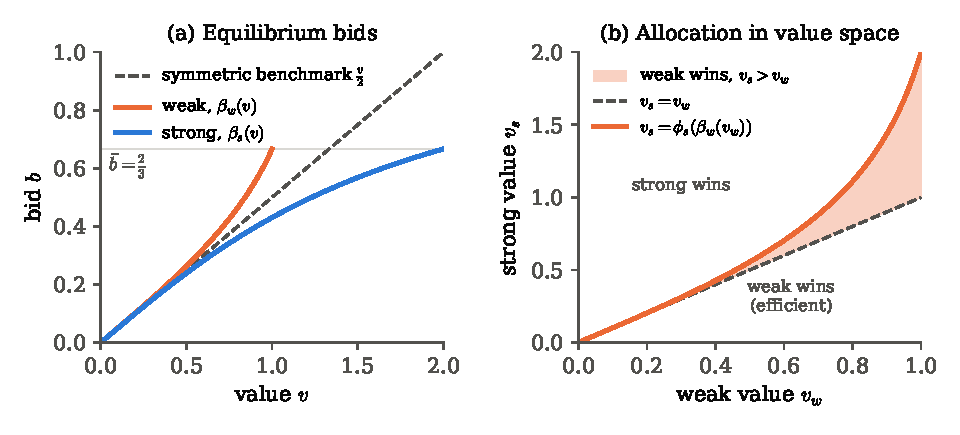
\includegraphics[width=\textwidth]{figures/ch14/asym_bids.pdf}
\caption{Asymmetric first-price auction with $V_w\sim U[0,1]$ and $V_s\sim U[0,2]$. Panel (a): the
equilibrium bid functions \eqref{eq:14-unif-beta} and the symmetric benchmark $\frac{v}{2}$. Both
bidders' bids end at the common top bid $\bar b=\frac{2}{3}$. Panel (b): the weak bidder wins below
the curve $v_s=\phi_s(\beta_w(v_w))$. In the shaded band between that curve and the diagonal the weak
bidder wins although the strong bidder values the object more.}
\label{fig:14-asym-bids}
\end{figure}

The example shows every effect of \cref{prop:14-maskin-riley}. The strong bidder's payoff falls by
$0.0764$ when we move from the second-price to the first-price auction. The weak bidder's payoff
rises by $0.0136$, and total surplus falls by $0.0205$. Revenue is total surplus minus payoffs, so
revenue rises by $0.0764-0.0136-0.0205=0.0423$. The first-price auction extracts more from the strong
bidder than it gives away to the weak bidder and to inefficiency.

\subsection{Revenue comparisons with asymmetric bidders}\label{sec:14-asym-revenue}

The decomposition used in the example holds in general:
\begin{equation}\label{eq:14-rev-decomp}
\text{expected revenue}=\text{expected total surplus}-\sum_i\E\bigl[\pi_i(V_i)\bigr].
\end{equation}
Moving from the open auction to the first-price auction lowers total surplus, by
\cref{prop:14-maskin-riley}(iii). It raises the weak bidder's rents and lowers the strong bidder's
rents, by part (iv). The net effect on revenue has no general sign.
\citet{MaskinRiley2000} give sufficient conditions on the value distributions under which the
first-price auction yields higher revenue, and others under which the open auction does. In the
uniform example the first-price auction raises more revenue. \citet[Section II.D]{AtheyLevinSeira2011} stress that ``there is no general theoretical
comparison of expected revenue, even with fixed participation.''

The optimal auction of \cref{sec:14-optimal} explains why the first-price auction often does well.
In the same example, \cref{sec:14-optimal-asym} showed that the optimal mechanism of
\citet{Myerson1981} gives the weak bidder a head start of $\frac{1}{2}$, because $\psi_w(v)=2v-1$
exceeds $\psi_s(v)=2v-2$ at every value. It earns $\frac{31}{48}\approx 0.646$, well above both
standard formats. The first-price auction tilts the allocation in the same direction as the optimal
mechanism, without design, and it captures part of the gain.
\citet[Section 7]{AtheyHaile2007} summarize the trade-off. First-price auctions may allocate
inefficiently with asymmetric bidders, but they ``tend to raise more revenue in private values
settings.''

\section{Participation and Entry}\label{sec:14-entry}

So far the set of bidders has been fixed. In practice, bidding is costly. A timber bidder must cruise
the tract to estimate its volume and quality, and a construction firm must prepare a detailed cost
estimate. Firms decide whether to incur these costs before the auction. The number of bidders is then
an equilibrium outcome, and the auction format can affect it.

Two timing assumptions organize the theory. In the first, a bidder knows its value before deciding
whether to pay the entry cost. In the second, a bidder learns its value only after paying the cost.
\citet{Samuelson1985} studies the first timing, and \citet{LevinSmith1994} study the second. The
second timing underlies the empirical work of \citet{AtheyLevinSeira2011}, where the entry cost is
the cost of cruising the tract. The two timings give the entry cost different meanings
\citep[Section~2.2, p.~91]{HortacsuPerrigne2021}. When bidders know their values, entry is
\emph{selective}, since only bidders with high enough values enter, and $K$ is a cost of preparing a
bid. When bidders learn their values after entry, entry is \emph{nonselective}, and $K$ also covers
the cost of acquiring information. \citet{RobertsSweeting2016} nest both cases. In their model each
potential bidder observes a noisy signal of its value before it decides whether to enter. The model
of \citet{LevinSmith1994} is the case of signals independent of values, and the model of
\citet{Samuelson1985} is the case of perfect correlation \citep[footnote~9, p.~92]{HortacsuPerrigne2021}.
Throughout this section, $K>0$ is the entry cost, $N$ is the number
of potential bidders, and $p$ denotes an entry probability. Elsewhere $p$ is the clock price
(\cref{sec:14-formats}) or a probability of winning (\cref{sec:14-ret-selfselection}).

\subsection{Entry with values known in advance}\label{sec:14-entry-samuelson}

Suppose each of $N$ symmetric potential bidders knows its value $v_i$, drawn independently from $F$
on $[\underline v,\bar v]$. A bidder who pays $K$ may bid in a standard auction with reserve price
$r$. We look for a symmetric equilibrium in which a bidder enters if and only if its value is at least
a cutoff $v^*$.

The cutoff type is pinned down by a simple observation. A bidder with value $v^*$ wins only if no
rival enters, because any entrant has a value above $v^*$. That happens with probability
$F(v^*)^{N-1}$, and then the lone bidder pays the reserve price. In the second-price auction this is
immediate. In the first-price auction the cutoff type also bids $r$, because it wins only when it is
alone and any higher bid would only raise its payment. Indifference of the cutoff type requires
\begin{equation}\label{eq:14-samuelson-cutoff}
(v^*-r)\,F(v^*)^{N-1}=K .
\end{equation}
Let $\Phi(v)=(v-r)F(v)^{N-1}$. It is zero at $v=r$ and strictly increasing, with
$\Phi'(v)=F(v)^{N-1}+(v-r)(N-1)F(v)^{N-2}f(v)>0$. So a unique interior cutoff exists whenever $\bar
v-r>K$. Types above $v^*$ strictly prefer to enter, because a bidder's expected surplus rises with its
value at the rate of its win probability.

Implicit differentiation of \eqref{eq:14-samuelson-cutoff} gives the comparative statics:
\[
\frac{dv^*}{dK}=\frac{1}{\Phi'(v^*)}>0,\qquad
\frac{dv^*}{dr}=\frac{F(v^*)^{N-1}}{\Phi'(v^*)}\in(0,1),\qquad
\frac{dv^*}{dN}=-\frac{(v^*-r)F(v^*)^{N-1}\ln F(v^*)}{\Phi'(v^*)}>0,
\]
where the last expression treats $N$ as continuous. The entry cost and the reserve price both screen
out low-value bidders. A higher reserve raises the cutoff by less than one for one. The entry cost
differs from a reserve price in one respect. It is a resource cost borne by every entrant, and the
seller collects none of it.

\begin{example}[Cutoffs with uniform values]\label{ex:14-samuelson}
Let $F$ be uniform on $[0,1]$, $N=5$ and $r=0$. Equation \eqref{eq:14-samuelson-cutoff} becomes
$(v^*)^5=K$, so $v^*=K^{\frac{1}{5}}$. With $K=0.05$ the cutoff is $0.549$, each potential bidder
enters with probability $0.451$, and $2.25$ bidders enter on average. With $K=0.10$ the cutoff is
$0.631$ and $1.85$ bidders enter on average. Raising the reserve to $r=0.25$ raises the cutoffs to
$0.610$ and $0.690$. These values come from \texttt{entry\_example.py}.
\end{example}

With values known in advance, the entrants are a selected sample of high-value bidders. This
complicates both theory and estimation. \citet[Section II.F]{AtheyLevinSeira2011} note that with
asymmetric bidders who have prior private information, ``the ex ante rankings of strong and weak
bidders may fail to hold conditional on entry.'' This is one reason they adopt the second timing.

\subsection{Entry with values learned after entry: the Levin-Smith model}\label{sec:14-entry-ls}

Now suppose a bidder learns its value only after paying $K$. Before entry, all $N$ potential bidders
are identical. Entrants observe the number of other entrants before bidding
\citep[Section 6.3.2]{AtheyHaile2007}. Let $\pi(k)$ be the expected profit, gross of $K$, of an
entrant when $k$ bidders enter in total, so that it faces $k-1$ rivals. We study the symmetric
equilibrium in which each potential bidder enters with probability $p$.

Given that the other $N-1$ potential bidders each enter with probability $p$, the number of rival
entrants is binomial. An entrant's ex ante expected profit is therefore
\begin{equation}\label{eq:14-entry-indiff}
\Pi(p)=\sum_{k=1}^{N}\binom{N-1}{k-1}p^{k-1}(1-p)^{N-k}\,\pi(k).
\end{equation}
A potential bidder enters with probability one if $\Pi(p)>K$, stays out if $\Pi(p)<K$, and is willing
to randomize if $\Pi(p)=K$.

\begin{lemma}\label{lem:14-pi-decreasing}
In the symmetric private values model with any standard auction and reserve price $r$, the gross
profit of an entrant is
\begin{equation}\label{eq:14-pik}
\pi(k)=\int_r^{\bar v}F(t)^{k-1}\bigl(1-F(t)\bigr)dt ,
\end{equation}
which is strictly decreasing in $k$. With values uniform on $[0,1]$ and $r=0$,
$\pi(k)=\frac{1}{k(k+1)}$.
\end{lemma}

\begin{proof}
By revenue equivalence, an entrant's interim surplus is the same in every standard auction. By
\cref{lem:14-ic}, a type $v\ge r$ facing $k-1$ rivals earns $\int_r^vF(t)^{k-1}dt$, and types below
$r$ earn zero. Taking expectations and exchanging the order of integration,
\[
\pi(k)=\int_r^{\bar v}\left[\int_r^{v}F(t)^{k-1}dt\right]f(v)\,dv
=\int_r^{\bar v}F(t)^{k-1}\left[\int_t^{\bar v}f(v)\,dv\right]dt
=\int_r^{\bar v}F(t)^{k-1}\bigl(1-F(t)\bigr)dt .
\]
Since $F(t)<1$ on the interior of the support, the integrand falls strictly in $k$. In the uniform
case, $\pi(k)=\int_0^1t^{k-1}(1-t)\,dt=\frac{1}{k}-\frac{1}{k+1}=\frac{1}{k(k+1)}$.
\end{proof}

\begin{proposition}[Symmetric entry equilibrium]\label{prop:14-ls-unique}
Suppose $\pi(k)$ is strictly decreasing in $k$ and $N\ge 2$. Then $\Pi(p)$ is strictly decreasing in
$p$, and there is a unique symmetric entry equilibrium $p^*$. If $\pi(N)\ge K$, then $p^*=1$. If
$\pi(1)\le K$, then $p^*=0$. Otherwise $p^*\in(0,1)$ solves $\Pi(p^*)=K$.
\end{proposition}

\begin{proof}
Let $X\sim\text{Binomial}(N-1,p)$ be the number of rival entrants, so $\Pi(p)=\E[\pi(1+X)]$. A
binomial random variable is stochastically increasing in its success probability. Since $\pi$ is
strictly decreasing, $\E[\pi(1+X)]$ is strictly decreasing in $p$. The function is continuous, with
$\Pi(0)=\pi(1)$ and $\Pi(1)=\pi(N)$. The three cases follow from the intermediate value theorem and
strict monotonicity.
\end{proof}

When $p^*\in(0,1)$, entrants earn zero expected profit net of the entry cost. This has a striking
consequence. Let the seller value the object at $v_0$, and let $S(k)$ be the expected gain from trade
when $k$ bidders enter, measured relative to the seller keeping the object. It equals the expected
value of the winner minus $v_0$ when a sale occurs, and zero otherwise. The seller's expected gain,
revenue minus $v_0$ times the probability of sale, equals expected gains from trade minus bidders'
expected gross rents. Gross rents sum to $Np^*\Pi(p^*)=Np^*K$. Hence
\begin{equation}\label{eq:14-ls-revenue}
\text{seller's expected gain}=\E\bigl[S(X^*)\bigr]-Np^*K,\qquad X^*\sim\text{Binomial}(N,p^*).
\end{equation}
The right side is expected social welfare. The seller captures all of the social surplus, net of
entry costs. With $v_0=0$ the seller's gain is its expected revenue.

\begin{proposition}[Levin and Smith 1994]\label{prop:14-ls-welfare}
Consider symmetric private values, a seller who values the object at $v_0$, and an efficient standard
auction with reserve price $r=v_0$. Then:
\begin{enumerate}[label=(\roman*)]
\item Social welfare $W(p)=\E[S(X)]-NpK$, with $X\sim\text{Binomial}(N,p)$, satisfies
$W'(p)=N\bigl(\Pi(p)-K\bigr)$. The equilibrium entry probability maximizes welfare among symmetric
entry probabilities.
\item If $p^*\in(0,1)$ at $r=v_0$, no reserve price gives the seller a higher expected gain than
$r=v_0$.
\end{enumerate}
\end{proposition}

\begin{proof}
(i) Write $X=\sum_{j=1}^{N}\epsilon_j$ with independent entry indicators $\epsilon_j$ that equal one
with probability $p_j$. Differentiating $\E[S(X)]$ with respect to $p_j$ gives
$\E[S(Y_{-j}+1)-S(Y_{-j})]$, where $Y_{-j}$ counts the other entrants. At $p_j=p$ for all $j$,
summing over $j$ yields
\[
\frac{d}{dp}\E[S(X)]=N\,\E\bigl[S(Y+1)-S(Y)\bigr],\qquad Y\sim\text{Binomial}(N-1,p).
\]
With $r=v_0$ and an efficient auction, $S(k)=\E\bigl[(\max\{V_1,\dots,V_k\}-v_0)^+\bigr]$. The
increment $S(k+1)-S(k)$ is then the expected marginal contribution of one more bidder,
$\E\bigl[(V_{k+1}-\max\{V_1,\dots,V_k,v_0\})^+\bigr]$. In a second-price auction with reserve $v_0$,
this is exactly the bidder's expected surplus when it faces $k$ rivals, which is $\pi(k+1)$. By
revenue equivalence the same holds in any efficient standard auction with reserve $v_0$. Therefore
$\frac{d}{dp}\E[S(X)]=N\,\E[\pi(Y+1)]=N\,\Pi(p)$, and $W'(p)=N(\Pi(p)-K)$. Since $\Pi$ is decreasing,
$W$ is concave, and its maximizer over $[0,1]$ is the $p^*$ of \cref{prop:14-ls-unique}.

(ii) Let $R(r)$ and $W_r(p)$ denote the seller's expected gain and welfare with reserve $r$, and let
$p^*(r)$ be the equilibrium entry probability. Net bidder rents are never negative in equilibrium, so $R(r)\le
W_r(p^*(r))$. For any fixed $p$, the reserve $v_0$ allocates the object efficiently among the
entrants and the seller, so $W_r(p)\le W_{v_0}(p)$. By part (i), $W_{v_0}(p)\le W_{v_0}(p^*(v_0))$.
Finally, \eqref{eq:14-ls-revenue} gives $W_{v_0}(p^*(v_0))=R(v_0)$ when $p^*(v_0)\in(0,1)$. Chaining
the inequalities, $R(r)\le R(v_0)$.
\end{proof}

Part (ii) reverses the logic of \cref{cor:14-optimal-reserve}. With a fixed number of bidders, the
seller sets a reserve above its own value to extract rents. With endogenous entry and zero expected
rents, there are no rents left to extract. A reserve above $v_0$ then only discourages entry and
distorts the allocation. \citet[Section~2.2, p.~91]{HortacsuPerrigne2021} state the contrast between
the two entry models. Under nonselective entry of the Levin-Smith type, the optimal reserve price is
the seller's own value. Under selective entry it is given by the formula \eqref{eq:14-optimal-reserve}
of the fixed-participation model. The proofs here are our own.
\citet{LevinSmith1994} also show that the random entry of the mixed
equilibrium wastes resources. Sometimes too many bidders enter and sometimes too few. A seller who
could limit the number of potential bidders, and charge an entry fee if needed, would earn more.

\begin{example}[Levin-Smith entry with uniform values]\label{ex:14-ls}
Let values be uniform on $[0,1]$, $r=v_0=0$ and $N=5$. By \cref{lem:14-pi-decreasing},
$\pi(1),\dots,\pi(5)=\frac{1}{2},\frac{1}{6},\frac{1}{12},\frac{1}{20},\frac{1}{30}$, so
$\Pi(1)=\pi(5)=\frac{1}{30}\approx 0.033$. Every entry cost between $\frac{1}{30}$ and $\pi(1)=\frac{1}{2}$ therefore
produces a mixed equilibrium. For $K\ge\frac{1}{2}$ nobody enters. With $K=0.05$, solving $\Pi(p)=K$ numerically gives $p^*=0.816$, so $4.08$
bidders enter on average. Expected revenue equals expected welfare, $0.592$. With $K=0.10$, $p^*=0.559$,
$2.79$ bidders enter on average, nobody enters with probability $0.017$, and revenue is $0.425$.
\Cref{fig:14-entry}(a) shows the two solutions.

The value of limiting entry is visible in \cref{fig:14-entry}(b). With $K=0.05$ and $N=4$ potential
bidders, $\pi(4)=\frac{1}{20}=K$, so all four enter and revenue is $\frac{3}{5}=0.600$. Adding a fifth
potential bidder lowers revenue to $0.592$, and ten potential bidders lower it to $0.574$. With
$K=0.10$, revenue peaks at $0.452$ with $N=3$. The losses are modest here, but they have the sign
that \citet{LevinSmith1994} emphasize. All numbers come from \texttt{entry\_example.py}.
\end{example}

\begin{figure}[htbp]
\centering
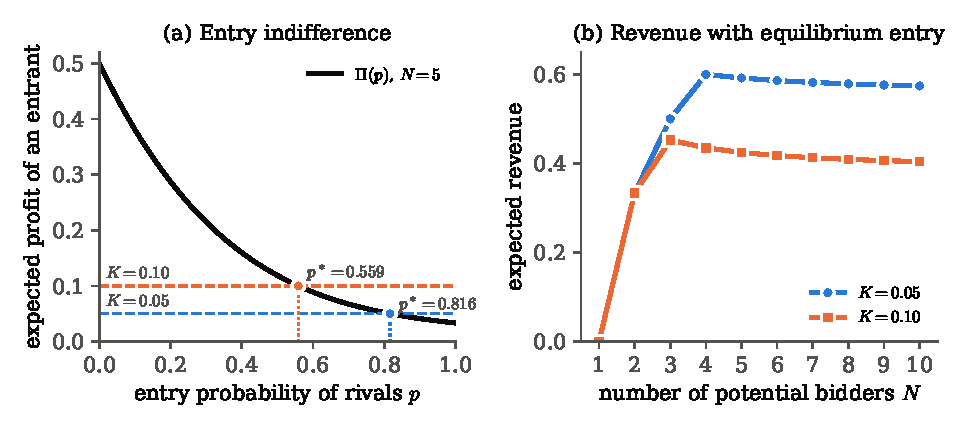
\includegraphics[width=\textwidth]{figures/ch14/entry.pdf}
\caption{Levin-Smith entry with uniform values and no reserve price. Panel (a): the ex ante profit of
an entrant $\Pi(p)$ in \eqref{eq:14-entry-indiff} for $N=5$, and the equilibrium entry probabilities
for $K=0.05$ and $K=0.10$. Panel (b): expected revenue in the symmetric entry equilibrium as a
function of the number of potential bidders $N$.}
\label{fig:14-entry}
\end{figure}

\subsection{Asymmetric bidders and type-symmetric entry equilibria}\label{sec:14-entry-als}

\citet{AtheyLevinSeira2011} combine the Levin-Smith timing with the asymmetric model of
\cref{sec:14-asym}. There are $N_L$ potential loggers with value distribution $F_L$ and $N_M$
potential mills with value distribution $F_M$. Mills are strong: $F_M$ dominates $F_L$ in the
reverse hazard rate order. Each firm decides independently whether to pay $K$, learns its value if it
does, and learns which rivals entered before bidding \citep[Section II.A]{AtheyLevinSeira2011}.

The model omits two features that could also matter for the format comparison. Bidders may have a
common value component, from private estimates of timber quality and volume or from differing
beliefs about future market conditions. They may also be risk averse. \citet[Section
II.F]{AtheyLevinSeira2011} abstract from both for two reasons. The format differences they observe
are qualitatively different from those that common values or risk aversion would imply, and
including either feature significantly complicates the analysis. They also restrict attention to
type-symmetric equilibria, which they regard as a convenient assumption that allows point
identification of entry costs.

Let $\pi_L^\tau(n_L,n_M)$ and $\pi_M^\tau(n_L,n_M)$ be the expected profits, gross of $K$, of a
participating logger and mill in format $\tau\in\{\mathrm{o},\mathrm{s}\}$ (open or sealed). The superscript $\tau$ indexes the format
and is unrelated to the payment rule $\tau_i$ of \cref{sec:14-ret}. The
participants are $n_L$ loggers and $n_M$ mills, and these counts include the bidder itself. Following
\citet[eq.~(4)]{AtheyLevinSeira2011}, bidder $i$'s ex ante profit from entering is
\begin{equation}\label{eq:14-als-exante}
\Pi_i^\tau(\bm p)=\sum_{\bm n}\pi_i^\tau(n_L,n_M)\,\Pr\bigl[n_L,n_M\mid i\text{ enters, rivals play }\bm p_{-i}\bigr],
\end{equation}
where $\bm p$ is the profile of entry probabilities. When all loggers enter with probability $p_L$ and
all mills with probability $p_M$, the probabilities are binomial. Write
$\mathrm{bin}(k;m,p)=\binom{m}{k}p^k(1-p)^{m-k}$. For a logger and a mill, respectively,
\begin{align}
\Pi_L^\tau(p_L,p_M)&=\sum_{n_L=1}^{N_L}\sum_{n_M=0}^{N_M}\mathrm{bin}(n_L-1;N_L-1,p_L)\,\mathrm{bin}(n_M;N_M,p_M)\,\pi_L^\tau(n_L,n_M),\label{eq:14-als-PiL}\\
\Pi_M^\tau(p_L,p_M)&=\sum_{n_L=0}^{N_L}\sum_{n_M=1}^{N_M}\mathrm{bin}(n_L;N_L,p_L)\,\mathrm{bin}(n_M-1;N_M-1,p_M)\,\pi_M^\tau(n_L,n_M).\label{eq:14-als-PiM}
\end{align}

\begin{definition}[Type-symmetric entry equilibrium]\label{def:14-type-symmetric}
A \emph{type-symmetric entry equilibrium} \citep[Section II.A]{AtheyLevinSeira2011} consists of bid
strategies $b_L(\cdot;\bm n)$, $b_M(\cdot;\bm n)$ and entry probabilities $p_L$, $p_M$ with three
properties.
\begin{enumerate}[label=(\roman*)]
\item All loggers use $(b_L,p_L)$ and all mills use $(b_M,p_M)$.
\item Each bidder's bid strategy maximizes its profit conditional on entering, for every set of
participants.
\item Each bidder enters if and only if its expected profit from entry \eqref{eq:14-als-exante} is at
least $K$. It may randomize when the two are equal.
\end{enumerate}
\end{definition}

Bid strategies in the open auction are $b_k(v;\bm n)=v$. In the sealed auction they solve
\eqref{eq:14-ts-foc-L} and \eqref{eq:14-ts-foc-M} with $b_k(r;\bm n)=r$. A type-symmetric entry
equilibrium exists in both formats, but it need not be unique \citep[Section
II.C]{AtheyLevinSeira2011}. The following condition, with at least two potential bidders of each
type, restores uniqueness. For the proof we maintain
that a participant's expected profit falls when a rival is added, strictly in expectation. In the
open auction this holds auction by auction, since a bidder's surplus
$(v-\max\{\text{rival values},r\})^+$ can only fall when a rival is added.

\begin{proposition}[Athey, Levin and Seira 2011, Proposition 1]\label{prop:14-als-unique}
Suppose that for all $n_L,n_M$,
\begin{equation}\label{eq:14-als-condition}
\pi_M^{\mathrm{s}}(n_L,n_M+1)>\pi_L^{\mathrm{s}}(n_L,n_M).
\end{equation}
Then every type-symmetric entry equilibrium of either auction format has $p_L=0$ or $p_M=1$. If
also $N_L\ge 2$ and $N_M\ge 2$, each format has a unique type-symmetric entry equilibrium.
\end{proposition}

Condition \eqref{eq:14-als-condition} compares a mill and a logger that face the same $n_M$ mills.
The mill faces $n_L$ loggers, while the logger faces only $n_L-1$ other loggers. The condition
requires the mill to earn more despite its extra rival. In the words of \citet[Section
II.C]{AtheyLevinSeira2011}, ``mills have a sufficient value advantage over loggers to outweigh the
effects of facing an additional bidder.'' They call the condition ``rather strong'' as theory, and
they verify it for every tract in their estimated model (\cref{ch:auction-empirics}).

\begin{proof}[Proof sketch]
\emph{Mills earn more than loggers at every entry profile.} Fix $(p_L,p_M)$. A logger who enters
faces $X_L\sim\text{Binomial}(N_L-1,p_L)$ other loggers and $X_M\sim\text{Binomial}(N_M,p_M)$ mills. A
mill who enters faces $X_L+\epsilon_L$ loggers and $X_M-\epsilon_M$ other mills. Here $\epsilon_L$ is an
indicator with success probability $p_L$, independent of everything else, and $\epsilon_M$ is the entry
indicator of one of the $N_M$ mills counted in $X_M$. Then $X_L+\epsilon_L\sim\text{Binomial}(N_L,p_L)$
and $X_M-\epsilon_M\sim\text{Binomial}(N_M-1,p_M)$, as a mill's counts require. Using monotonicity, then \eqref{eq:14-als-condition}, then monotonicity again,
\[
\pi_M(X_L+\epsilon_L,\,X_M-\epsilon_M+1)\ \ge\ \pi_M(X_L+1,\,X_M-\epsilon_M+1)\ >\
\pi_L(X_L+1,\,X_M-\epsilon_M)\ \ge\ \pi_L(X_L+1,\,X_M).
\]
Taking expectations gives $\Pi_M(p_L,p_M)>\Pi_L(p_L,p_M)$ for every profile.

\emph{Either $p_L=0$ or $p_M=1$.} If loggers enter with positive probability, then $\Pi_L\ge K$. The
previous step gives $\Pi_M>K$, so mills enter with probability one.

\emph{Uniqueness.} Candidate equilibria have either $p_M=1$ and $p_L$ solving the logger's condition,
or $p_L=0$ and $p_M<1$ solving the mill's condition. With all mills entering, a logger's payoff is
$\Pi_L(p_L,1)=\E[\pi_L(1+X_L,N_M)]$. When $N_L\ge 2$, the count $X_L$ of other loggers is
stochastically increasing in $p_L$, so $\Pi_L(\cdot,1)$ is strictly decreasing. When $N_M\ge 2$, the
same argument shows that $\Pi_M(0,\cdot)$ is strictly decreasing. Each family therefore has at most
one member. Suppose an equilibrium with $p_L=0$
and $p_M<1$ exists. Then $\Pi_M(0,p_M)\le K$ when $p_M=0$, or $\Pi_M(0,p_M)=K$ when $p_M>0$. In
either case $\Pi_M(p_L,1)\le\Pi_M(0,1)<\Pi_M(0,p_M)\le K$ for every $p_L$, so no equilibrium with
$p_M=1$ exists. Only one candidate survives.

\emph{Both formats.} For any participant set, mills earn more and loggers less in the open auction
than in the sealed auction \citep[Section II.D]{AtheyLevinSeira2011}. This is the many-bidder
analogue of \cref{prop:14-maskin-riley}(iv). Hence
$\pi_M^{\mathrm{o}}(n_L,n_M+1)\ge\pi_M^{\mathrm{s}}(n_L,n_M+1)>\pi_L^{\mathrm{s}}(n_L,n_M)\ge\pi_L^{\mathrm{o}}(n_L,n_M)$,
and the argument applies to the open auction as well.
\end{proof}

\citet{AtheyLevinSeira2011} state uniqueness without the restriction $N_L,N_M\ge 2$, and the
restriction matters. With a single potential logger, $\Pi_L(p_L,1)=\pi_L(1,N_M)$ does not depend on
$p_L$. If $K=\pi_L(1,N_M)$, the logger is indifferent at every $p_L$, and mills strictly prefer to
enter by the first step of the proof. Every profile $(p_L,1)$ with $p_L\in[0,1]$ is then an
equilibrium. With one mill and one logger in the sealed auction of \cref{ex:14-als-entry} below, this
happens at $K=\pi_L^{\mathrm{s}}(1,1)=0.0969$. A single potential mill creates the same indifference at
$K=\pi_M(0,1)$, the profit of a mill without rivals, where every profile $(0,p_M)$ is an equilibrium.
At every other entry cost, a payoff that does not depend on its own type's entry probability is either
above or below $K$. It then pins down a single entry probability, and the equilibrium is again unique.
The separation result, $p_L=0$ or $p_M=1$, holds for any numbers of potential bidders.

The empirically relevant equilibrium has every mill entering and loggers randomizing,
$p_M=1$ and $p_L\in(0,1)$. \citet[Section II.C]{AtheyLevinSeira2011} motivate this case with their
data: they ``observe logger entry in more than 85\% of sales and always more potential logger
entrants than actual logger entrants.''

\casehead{The homogeneous benchmark}
If $F_L=F_M$, every bidder is the same and revenue equivalence applies conditional on the number of
entrants. Each format then produces the same $\pi(k)$, given by \eqref{eq:14-pik}, and the same
entry condition. \citet[Section II.D]{AtheyLevinSeira2011} conclude that the two formats have
``(i) the same expected entry, (ii) the same allocation, and (iii) the same expected revenue.''
Format differences in entry therefore require asymmetric bidders.

\begin{proposition}[Athey, Levin and Seira 2011, Proposition 2]\label{prop:14-entry-format}
For any type-symmetric entry equilibrium of the sealed bid auction, there is a type-symmetric entry
equilibrium of the open auction with the following properties.
\begin{enumerate}[label=(\roman*)]
\item Loggers are less likely to enter.
\item Mills are more likely to enter.
\item It is less likely that a logger wins.
\end{enumerate}
\end{proposition}

\begin{proof}[Proof sketch for the empirically relevant case]
Assume \eqref{eq:14-als-condition} and $N_L,N_M\ge 2$, so each format has a unique equilibrium by
\cref{prop:14-als-unique}, and suppose the sealed
equilibrium has $p_M^{\mathrm{s}}=1$ and $p_L^{\mathrm{s}}\in(0,1)$. For every participant set, a
logger earns weakly less in the open auction. Hence $\Pi_L^{\mathrm{o}}(p_L,1)\le\Pi_L^{\mathrm{s}}(p_L,1)$
for every $p_L$. At $p_L^{\mathrm{s}}$ the sealed condition holds with equality, so
$\Pi_L^{\mathrm{o}}(p_L^{\mathrm{s}},1)\le K$. Because $\Pi_L^{\mathrm{o}}(\cdot,1)$ is decreasing,
the open-auction solution satisfies $p_L^{\mathrm{o}}\le p_L^{\mathrm{s}}$. This is (i). Mills earn
weakly more in the open auction and face fewer loggers, so
$\Pi_M^{\mathrm{o}}(p_L^{\mathrm{o}},1)\ge\Pi_M^{\mathrm{s}}(p_L^{\mathrm{s}},1)\ge K$. Mills still enter
with probability one, which gives (ii) with equality. For (iii), two effects reinforce each other.
For a fixed set of participants, a logger wins less often in the open auction, which is efficient,
than in the sealed auction, by \cref{prop:14-maskin-riley}(iii). In the open auction, fewer logger
entrants also mean a lower chance that the highest value belongs to a logger.
\end{proof}

The general statement allows multiple equilibria, which is why it is phrased as existence of a
suitable open-auction equilibrium. Under the conditions of \cref{prop:14-als-unique}, the prediction
is sharp: ``open
bidding leads to less logger entry, equivalent mill entry and a lower chance that a logger wins''
\citep[Section II.D]{AtheyLevinSeira2011}. The revenue comparison remains ambiguous. Sealed bidding
attracts more loggers, which raises competition, but it allocates inefficiently. The sealed auction is
``inefficient even conditional on participation,'' while the efficient type-symmetric outcome is an
equilibrium of the open auction \citep[Section II.D, citing \citealp{AtheyLevinSeira2004}]{AtheyLevinSeira2011}. The idea that sealed bids
encourage entry by weaker bidders is emphasized by \citet{Klemperer2004} in the context of spectrum
auctions \citep[footnote~4, p.~215]{AtheyLevinSeira2011}. \citet[Section~7]{AtheyHaile2007} likewise
list entry among the factors that govern the choice of format. The format ``also affects bidder entry
when bidders are asymmetric,'' and they cite \citet{Klemperer2002} and \citet{AtheyLevinSeira2004}. The
mechanism is the one of \cref{prop:14-entry-format}. An ascending auction deters entry by bidders who
expect to be outbid by a stronger rival.
\citet{Klemperer2002} proposes hybrid formats that end with a sealed-bid stage.

\begin{example}[One mill and one potential logger]\label{ex:14-als-entry}
Take the values of \cref{ex:14-asym-uniform}: the mill draws from $U[0,2]$, the logger from
$U[0,1]$, and $r=0$. With both present, \cref{tab:14-asym-example} gives
$\pi_L^{\mathrm{s}}=0.0969$, $\pi_L^{\mathrm{o}}=\frac{1}{12}\approx 0.0833$,
$\pi_M^{\mathrm{s}}=0.5069$ and $\pi_M^{\mathrm{o}}=\frac{7}{12}$. A mill alone pays the reserve and
earns $\E[V_M]=1$, and a logger alone earns $\E[V_L]=\frac{1}{2}$. Condition
\eqref{eq:14-als-condition} holds, since $0.5069>0.5$. Let $K=0.09$. This cost differs from the
knife-edge values $\pi_L^\tau(1,1)$ and $\pi_M^\tau(0,1)=1$ of both formats, so each format has a
unique type-symmetric entry equilibrium. In the sealed auction the mill
enters and the logger enters too, because $0.0969>0.09$. Revenue is $0.459$, the logger wins with
probability $\frac{1}{3}$, and welfare is $1.0628-2K=0.883$. In the open auction the logger stays
out, because $0.0833<0.09$. The mill wins at the reserve price, so revenue is zero and welfare is
$1-K=0.91$. The sealed auction raises far more revenue through entry, and the open auction is more
efficient.
\end{example}

The example is extreme because $r=0$, but it isolates the mechanism of \cref{prop:14-entry-format}.
The weak bidder's expected profit is higher under sealed bidding, so it enters more often. That entry
disciplines the strong bidder, whose price would otherwise be set by the reserve.

\casehead{From entry decisions to entry costs}
The indifference of randomizing bidders carries empirical content. For any bidder who randomizes,
expected profit from entry equals $K$. \citet[Section 6.3.2]{AtheyHaile2007} write this as
\begin{equation}\label{eq:14-entry-cost-id}
K=\sum_{\mathcal A:\,i\in\mathcal A}\Pr\bigl(\tilde{\mathcal N}=\mathcal A\mid i\in\tilde{\mathcal
N}\bigr)\,\pi_i(\mathcal A),
\end{equation}
where $\tilde{\mathcal N}$ is the random set of entrants. Here $\pi_i(\mathcal A)$ is bidder $i$'s
expected gross profit when the participant set is $\mathcal A$,
\begin{equation}\label{eq:14-entry-profit-id}
\pi_i(\mathcal A)=\E\Bigl[\bigl(V_i-\beta_i(V_i;\mathcal A)\bigr)\,G_{M_i|B_i}\bigl(\beta_i(V_i;\mathcal
A)\bigm|\beta_i(V_i;\mathcal A);\mathcal A\bigr)\Bigr],
\end{equation}
with $G_{M_i|B_i}$ the distribution of the highest rival bid given bidder $i$'s own bid. The notation
follows \citet[Section 6.3.2]{AtheyHaile2007}, who write $\Pi_i$ for what we call $\pi_i$. The post-entry profits are identified
from bids, and the entry probabilities are observed. The level of the entry cost is then identified
in dollars. This contrasts with entry models that infer profits only from entry decisions
\citep[Section 6.3.2]{AtheyHaile2007}. \Cref{ch:auction-empirics} develops the estimator.

\section{Collusion and the Choice of Format}\label{sec:14-collusion}

Collusion among bidders is a long-standing concern in auction design. Gifford Pinchot, the first
chief of the US Forest Service, advocated sealed bidding for timber. He described a sale on sealed
bids as ``thereby preventing the customary collusion between bidders'' \citep[p.~209]{Pinchot1998},
as quoted by \citet[footnote 2]{AtheyLevinSeira2011}. \citet[Section 9]{MilgromWeber1982} name the
same setting as a limit of their noncooperative theory. They judge it less reasonable for timber
rights on federal land, where ``the bidders (owners of lumber mills) are members of a trade
association and bid repeatedly against each other'' \citep[p.~1118]{MilgromWeber1982}. This section explains why the format matters for collusion. The
general theory of cartels is in \cref{ch:collusion-theory}, and prosecuted bidding rings are studied
in \cref{ch:collusion-evidence}.

\subsection{Rings in second-price and ascending auctions}\label{sec:14-collusion-open}

A \emph{bidding ring} is a group of bidders who agree to suppress competition among themselves.
Consider the private values model with a ring $\mathcal C\subset\mathcal N$ of $m\ge 2$ members.
Suppose for now that members know each other's values. The simplest agreement designates the member
with the highest value, bidder $d$, to bid. The other members abstain or bid the reserve price.
Bidders outside the ring bid as usual.

\begin{proposition}[Robinson 1985]\label{prop:14-robinson}
In a second-price or ascending auction with private values, the ring agreement in which the
highest-value member bids its value and the other members abstain is self-enforcing. No member gains
by deviating within the auction, whatever the values and whether or not the members meet again.
\end{proposition}

\begin{proof}
Outsiders bid their values, which is weakly dominant by \cref{prop:14-spa-dominant}. The designated
bidder $d$ bids $v_d$, which is also weakly dominant. Consider a member $j\neq d$, with $v_j\le v_d$.
Bidder $j$ wins only with a bid above $v_d$, since $d$ stays in until the price reaches $v_d$. A
winning deviation then pays at least $v_d\ge v_j$, so its payoff is at most zero. Abstaining yields
zero. Hence no deviation is profitable.
\end{proof}

The ring gains because it removes the price pressure that members exert on each other. Let
$V^{\mathcal C}_{(1)}\ge V^{\mathcal C}_{(2)}$ be the two highest member values and $V^{\mathcal O}_{(1)}$
the highest outsider value. Competitive bidding sets the price at the second-highest value overall.
Under the ring, the price is $\max\{V^{\mathcal O}_{(1)},r\}$ whenever a member wins. The price
falls only when the two highest values both belong to members, and then by
\begin{equation}\label{eq:14-ring-gain}
\Delta P=\Bigl(V^{\mathcal C}_{(2)}-\max\bigl\{V^{\mathcal O}_{(1)},r\bigr\}\Bigr)^+ .
\end{equation}
The ring does not change who wins, so the allocation stays efficient. The ring transfers surplus
from the seller to its members.

\Citet[Section~2.5, p.~96]{HortacsuPerrigne2021} draw the practical lesson from \cref{prop:14-robinson}.
Open auctions may favor collusion, because bidders meet face to face and can react at once to each
other's behavior. If the ring allocates the object to its highest-value member, no other member gains
by deviating, since that member can always outbid the deviator. For this reason auction theorists
recommend first-price auctions. The issue is practical. Collusion at U.S.\ Forest Service timber sales
was suspected in the 1970s, and it was the subject of allegations and of a congressional hearing in
1977, though few cases were prosecuted. In 1976 the federal government recommended first-price sealed
bids over ascending auctions, mainly to reduce collusion \citep[Section~2.4, p.~96]{HortacsuPerrigne2021}.
Sealed bids are no cure, however. The same survey reviews collusion in first-price procurement auctions
of construction contracts (their Section~3.4), and \cref{ch:collusion-evidence} studies such rings.

\subsection{Rings in first-price auctions}\label{sec:14-collusion-fpa}

The first-price auction is different. To gain, the designated bidder must bid less than the price
that competition would produce. Every other member with a value above that bid then has a unilateral
incentive to bid slightly more and win. In a one-shot auction, the designated bid must exceed the
values of all other members to deter such deviations. With known values, the ring must therefore pay
at least $V^{\mathcal C}_{(2)}$ whenever it wins. The price suppression of \eqref{eq:14-ring-gain}
cannot be sustained within a single sealed-bid auction.

Sustaining a first-price ring requires the threat of future punishment. A member who undercuts the
designated bidder is detected only after the bids are opened, and the ring can respond only in later
auctions. The agreement survives if the one-time gain from undercutting is smaller than the discounted
loss from the ring's collapse, a condition of the kind derived in \cref{ch:collusion-theory}. The
open auction needs no such condition. A deviation there is observed as it happens, and the designated
bidder answers it by continuing to bid. \citet[Section 7]{AtheyHaile2007} summarize the comparison:
first-price auctions ``may be less susceptible to collusion (detection and response to defections
are more difficult than in an ascending auction).'' This is why sealed bids appear in \cref{tab:14-ranking}
as the format less prone to collusion. \citet{Robinson1985} draws the policy conclusion that a seller
worried about rings should prefer the first-price format.

\subsection{Ring size, leakage and secret deviations}\label{sec:14-collusion-size}

The two formats also differ in who gains from a ring that does not include every bidder.
\citet[ch.~8, p.~176]{MarshallMarx2012} put the contrast as follows. In the ascending auction the
highest-value member stays in up to its value, exactly as it would without the ring. An outsider who
wins pays what it would have paid without collusion, so the ring captures all the gains. In the
sealed-bid auction the designated member bids strictly less than its noncollusive bid. Outsiders then
sometimes win auctions that they would have lost under competition. Part of the collusive gain spills
over to the outsiders, which \citet[p.~181]{MarshallMarx2012} call \emph{leakage}. The following example
computes the ascending-auction side of the comparison in closed form.

\begin{example}[Ring size with uniform values]\label{ex:14-ring-size}
Let $n$ bidders have values that are independent and uniform on $[0,1]$, with $r=v_0=0$. A ring of
$k\ge 1$ members bids in an ascending auction as in \cref{prop:14-robinson}, and the other $m=n-k$
bidders bid their values. We compute the expected price and the expected surplus of each bidder.

\emph{Step 1 (price reduction).} By \eqref{eq:14-ring-gain} with $r=0$, the ring lowers the price by
$(C_2-O_1)^+$. Here $C_2$ is the second-highest member value and $O_1$ the highest outsider value, with
$O_1=0$ when $m=0$. The density of $C_2$ is $k(k-1)x^{k-2}(1-x)$ on $[0,1]$, and $\Pr(O_1\le y)=y^m$.
For a fixed $x$,
\[
\E\bigl[(x-O_1)^+\bigr]=\int_0^x\Pr(O_1\le y)\,dy=\int_0^x y^m\,dy=\frac{x^{m+1}}{m+1}.
\]
Integrating over $C_2$ and using $k+m=n$,
\[
\E[\Delta P]=\frac{k(k-1)}{m+1}\int_0^1x^{n-1}(1-x)\,dx
=\frac{k(k-1)}{m+1}\left(\frac{1}{n}-\frac{1}{n+1}\right)
=\frac{k(k-1)}{(n-k+1)\,n\,(n+1)}.
\]

\emph{Step 2 (price).} Without a ring the expected price is $\E[V_{(n-1:n)}]=\frac{n-1}{n+1}$, so the
expected price with a ring of $k$ members is
\begin{equation}\label{eq:14-ring-price}
\E[P_k]=\frac{n-1}{n+1}-\frac{k(k-1)}{(n-k+1)\,n\,(n+1)}.
\end{equation}
With $k=2$ the fall is $\frac{2}{(n-1)n(n+1)}$.

\emph{Step 3 (surplus).} An outsider wins only with the highest value overall, and it then pays the
second-highest value overall, ring or no ring. Its expected surplus is therefore unchanged at
$\frac{1}{n}\E\bigl[V_{(n:n)}-V_{(n-1:n)}\bigr]=\frac{1}{n(n+1)}$. Members keep their competitive surplus
$\frac{k}{n(n+1)}$ and gain $\E[\Delta P]$ in addition. Per member,
\[
\frac{1}{k}\left[\frac{k}{n(n+1)}+\frac{k(k-1)}{(n-k+1)n(n+1)}\right]
=\frac{1}{n(n+1)}\cdot\frac{n}{n-k+1}
=\frac{1}{(n+1)(n-k+1)}.
\]
An all-inclusive ring, $k=n$, pays nothing, and each member earns $\frac{1}{n+1}=\frac{1}{n}\E[V_{(n:n)}]$.
\end{example}

\Cref{tab:14-mm-ring} reproduces Table~8.1 of \citet[ch.~8, p.~182]{MarshallMarx2012}, which compares
the two formats with five bidders. The ascending columns follow from \cref{ex:14-ring-size}. For
example, with $n=5$ and $k=3$, \eqref{eq:14-ring-price} gives $\frac{4}{6}-\frac{6}{3\cdot 30}=0.600$, and
each member earns $\frac{1}{6\cdot 3}\approx 0.056$. In the first-price auction the ring is a single
strong bidder whose value is the highest of $k$ uniform draws. That asymmetric auction has no closed
form. Marshall and Marx take its values from \citet[Table~III]{MarshallEtAl1994}, who compute them by
Monte Carlo with 100,000 draws.

\begin{table}[htbp]
\centering
\caption{Rings of different sizes with five bidders and uniform values}\label{tab:14-mm-ring}
\begin{tabular}{@{}ccccccc@{}}
\toprule
& \multicolumn{2}{c}{Expected price} & \multicolumn{2}{c}{Surplus per ring member} & \multicolumn{2}{c}{Surplus per outsider}\\
\cmidrule(lr){2-3}\cmidrule(lr){4-5}\cmidrule(l){6-7}
Ring size $k$ & Ascending & First price & Ascending & First price & Ascending & First price\\
\midrule
1 & 0.667 & 0.667 & 0.033 & 0.033 & 0.033 & 0.033\\
2 & 0.650 & 0.651 & 0.042 & 0.035 & 0.033 & 0.037\\
3 & 0.600 & 0.609 & 0.056 & 0.041 & 0.033 & 0.049\\
4 & 0.467 & 0.506 & 0.083 & 0.057 & 0.033 & 0.086\\
5 & 0.000 & 0.000 & 0.167 & 0.167 & -- & --\\
\bottomrule
\end{tabular}

\smallskip
\begin{minipage}{0.95\textwidth}
\footnotesize Notes: Five bidders with values independent and uniform on $[0,1]$, and a reserve price
of zero. A ring of size one means competitive bidding. The ascending columns and the first-price row
for $k=1$ are analytic. The other first-price entries are from \citet[Table~III]{MarshallEtAl1994}.
Source: \citet[ch.~8, Table~8.1, p.~182]{MarshallMarx2012}.
\end{minipage}
\end{table}

The table shows three effects. First, outsiders gain from a ring only in the sealed-bid auction. Their
surplus rises from 0.033 to 0.037, 0.049 and 0.086 as the ring grows from two to four members. Members
of a larger ring bid lower, and outsiders win more often and pay less \citep[p.~181]{MarshallMarx2012}.
The leakage also creates inefficiency. With a ring of four against one outsider, the outsider bids
about 0.40 when its value is about 0.54. The ring bids about 0.40 only when its highest value is about
0.76 \citep[pp.~183--184, using Figure~2 of \citealp{MarshallEtAl1994}]{MarshallMarx2012}. The outsider
then wins whenever the ring's highest value lies between 0.54 and 0.76.

Second, a ring that excludes some bidders hurts the seller more in the ascending auction. With two,
three and four members the expected price is 0.650, 0.600 and 0.467 there, against 0.651, 0.609 and
0.506 in the first-price auction. Each member also gains more, 0.042, 0.056 and 0.083 against 0.035,
0.041 and 0.057. In this example the incentive to collude is therefore stronger in the ascending auction
\citep[p.~181]{MarshallMarx2012}. Marshall and Marx stress in their footnote~21 that this ranking is not
a general result.

Third, leakage affects who wants to join. In the ascending auction there is no leakage, so outsiders
always want to join, and with symmetric bidders the ring wants to admit them
\citep[p.~177]{MarshallMarx2012}. In the sealed-bid auction an outsider may prefer to stay out. With
101 bidders, an outsider facing a ring of 99 earns 0.0159 in the first-price auction. As a member of a
ring of 100 it would earn only 0.0025. The last outsider facing a ring of 100 earns 0.0412, more than
the 0.0098 it would earn in the all-inclusive ring \citep[Table~8.2, pp.~185--186]{MarshallMarx2012}.
\Cref{ex:14-ring-size} reproduces their ascending entries, a member surplus of $\frac{1}{102\cdot
3}\approx 0.0033$, $\frac{1}{102\cdot 2}\approx 0.0049$ and $\frac{1}{102}\approx 0.0098$.

The same contrast governs enforcement. A \emph{secret deviation} is a clandestine bid at the main
auction, contrary to the ring's recommendation, that cannot be traced to the member without
substantial cost \citep[ch.~9, pp.~187--188]{MarshallMarx2012}. Secret deviations are a major concern
in sealed-bid auctions and a lesser one in ascending auctions. In the ascending auction the
highest-value member can stay active up to its value, as it would without the ring, so there is no
room for a profitable deviation. In the sealed-bid auction the designated member bids below its
noncooperative bid, which opens the door to deviations by other members. Marshall and Marx conclude
that pricing and enforcement structures are harder to implement in sealed-bid auctions, while the
structures for allocating the gains are much the same in the two formats \citep[p.~198]{MarshallMarx2012}.

\subsection{Knockouts and side payments}\label{sec:14-collusion-knockout}

The agreement above assumed that members know each other's values. In practice, a ring must elicit
values and divide the gains. Rings often hold a private auction among their members, called a
\emph{knockout}, before or after the real one. The winner of the knockout gets the object or the right to
bid for it, and side payments compensate the losers.

\citet{GrahamMarshall1987} study knockouts for second-price and English auctions.
In a knockout of the type they analyze, each member reports a value to a ring center. The highest
reporter bids its report in the main auction. If it wins at price $P$, it pays the center the amount
by which the second-highest report exceeds $P$. Its total outlay is
$P+(\hat z_{(2)}-P)^+=\max\{P,\hat z_{(2)}\}$, where $\hat z_{(2)}$ is the second-highest report. Each member thus
faces a second-price auction against the other reports and the outside bids, so truthful reporting is
weakly dominant. The center's collections are returned to members as transfers fixed in advance,
which keeps incentives intact and balances the budget in expectation.

\citet{McAfeeMcMillan1992} study rings in first-price auctions.
A \emph{weak cartel} cannot make side payments. Its best scheme has every member with a value above
the reserve bid the reserve price, with the winner chosen at random among them. A \emph{strong
cartel} can make side payments. It can allocate the object to the member with the highest value
through a first-price knockout whose winner pays its knockout bid to the other members in equal
shares.

\citet[ch.~9, pp.~191--192]{MarshallMarx2012} describe a strong cartel of this kind. From 1895 the
cast-iron pipe makers of the Addyston Pipe cartel met before each sealed-bid procurement in their pay
territories and held a knockout. The high bidder in the knockout was selected to bid at the
procurement. Its knockout bid was distributed among all the ring members, in shares that varied with
their production capacities \citep[p.~191, footnote~7]{MarshallMarx2012}. The other members either stayed
out or submitted deliberately losing bids. In one procurement in St.~Louis, Howard-Harrison won with a
bid of \$24, while Addyston and Dennis Long protected it with bids of \$24.37 and \$24.57. The
Chattanooga foundry could have supplied the pipe at \$17 or \$18 and still made a profit
\citep[p.~192]{MarshallMarx2012}. Marshall and Marx describe this mechanism in stylized form, and
their footnote~6 attributes the stylized model to \citet{McAfeeMcMillan1992}. The cartel thus ran a
version of the McAfee and McMillan knockout. With symmetric bidders that knockout lets the ring suppress
all competition among its members.

Knockouts used in practice need not be incentive compatible. \citet{Asker2010} studies a ring of eleven
wholesale stamp dealers that operated in the 1990s at ascending auctions, mainly at New York auction
houses \citep[ch.~9, p.~192]{MarshallMarx2012}. Before each auction the members reported values to a
ring center, in effect a sealed-bid knockout. The center bid for the member with the highest report,
and the other members stayed out. If the ring won, side payments depended on the reports and on the
price $P$ \citep[ch.~9, pp.~192--194]{MarshallMarx2012}. Rank the reports as $r_1>r_2>\dots>r_k>P$,
where member 1 is the winner and all other reports lie below $P$. Write $\rho_l=r_l$ for $l\le k$ and
$\rho_{k+1}=P$. Each increment $\rho_l-\rho_{l+1}$ with $2\le l\le k$ is split in half. The winner
keeps one half and pays out the other half, which is shared equally by the $l-1$ losing members whose
reports are at least $\rho_l$ \citep[p.~193]{MarshallMarx2012}. Losing member $j\in\{2,\dots,k\}$
therefore receives
\begin{equation}\label{eq:14-stamp-transfer}
t_j=\sum_{l=j}^{k}\frac{\rho_l-\rho_{l+1}}{2(l-1)},
\end{equation}
and members whose reports lie below $P$ receive nothing. These are the transfers of Table~9.1 of
\citet[p.~193]{MarshallMarx2012}. Summing over $j$ counts the term of increment $l$ once for each of
the $l-1$ members $j\le l$, so
\[
\sum_{j=2}^{k}t_j=\sum_{l=2}^{k}(l-1)\,\frac{\rho_l-\rho_{l+1}}{2(l-1)}=\sum_{l=2}^{k}\frac{\rho_l-\rho_{l+1}}{2}=\frac{\rho_2-P}{2}.
\]
The sum equals $\frac{r_2-P}{2}$ when at least one losing member reports more than $P$, and zero
otherwise. It is exactly the winner's payment in Table~9.1, so the rule balances the budget. Members with higher reports
receive larger payments. The rule also rewards overreporting. Only the term $l=j$ of
\eqref{eq:14-stamp-transfer} contains $r_j$. A losing member therefore raises its transfer at the rate
$\frac{1}{2(j-1)}$ by raising its report, as long as the report stays below $r_{j-1}$. A member whose
value lies below $P$ can likewise collect a share by reporting more than $P$. Marshall and Marx note, as
\citet{GrahamMarshallRichard1990} had pointed out, that such rules give members an incentive to
overreport. Inflated reports can lead the ring to win lots that an outsider valued more, at prices
above the ring's own highest value. In the model with unobserved heterogeneity, \citet[Section~VII.C and
Table~10]{Asker2010} estimates that this happened in 19 percent of the auctions the ring won.
\Cref{ch:collusion-evidence} analyzes this ring in detail.

A ring at ascending auctions where members can see who holds the high bid needs no communication
before the auction. Its members follow one rule. No member raises the bid when another member is the
current high bidder \citep[ch.~9, p.~194]{MarshallMarx2012}. The items that members win are then
reallocated at a knockout held after the auction. \citet[ch.~3, pp.~61--64]{MarshallMarx2012} give a
fictional account of such a ring at antique auctions, with footnotes that tie its features to known
cases. At the knockout, members submit \emph{bonus bids}, offers in excess of the price paid at the
main auction. The highest bonus bidder reimburses the member who bought the item and puts the bonus
``into the hat.'' The hat money is divided equally among the members at the end of the day. In their
example, ten members shared about \$500,000, or \$50,000 each. A ring whose members differ in strength
can run a \emph{nested knockout}. The three members of an inner ring do not bid against each other at
the first knockout. The items they win there go to a second knockout among the inner ring alone.
Suppose an inner member wins the first knockout with a bonus of \$5,000 and the second with a bonus of
\$10,000. The first amount is split among all ten members, and the second among the inner three
\citep[ch.~3, p.~63]{MarshallMarx2012}. Equal sharing
again invites overbidding. A member may raise the bonus on an item it does not want, because it
receives a share of every bonus. The cases behind the account include rings in antiques, used
industrial machinery and real estate \citep[ch.~3, p.~55, and ch.~9, p.~194]{MarshallMarx2012}.

\subsection{Collusion and entry: Athey, Levin and Seira's Proposition 3}\label{sec:14-collusion-als}

\citet[Section II.E]{AtheyLevinSeira2011} add collusion to the entry model of \cref{sec:14-entry}.
They cite a long record of concern about collusion in open Forest Service sales, including the
empirical study of oral timber auctions by \citet{BaldwinMarshallRichard1997}. Collusive schemes take
many forms, so they assume for concreteness that participating mills in an open auction cooperate
perfectly. ``The participating
mill with the highest value bids his value, while the other mills register as participants but do not
actively bid. Loggers simply bid up to their value.'' Entry decisions remain independent, so mills
anticipate cooperating with whichever mills enter but do not coordinate entry. We call this the
\emph{mill-collusive} open auction.

\begin{proposition}[Athey, Levin and Seira 2011, Proposition 3]\label{prop:14-collusion-open}
For any type-symmetric entry equilibrium of the open auction, there is a type-symmetric collusive
equilibrium with the following properties.
\begin{enumerate}[label=(\roman*)]
\item Loggers are less likely to enter.
\item Mills are more likely to enter.
\item It is less likely that a logger wins.
\end{enumerate}
Thus, for any type-symmetric entry equilibrium of the sealed bid auction, there is a type-symmetric
collusive equilibrium of the open auction in which properties (i) to (iii) hold. In the empirically
relevant case, with $p_M=1$ and $p_L\in(0,1)$, collusion leaves entry and the allocation unchanged and
only lowers prices.
\end{proposition}

\begin{proof}[Proof sketch]
\emph{Fixed participants.} The highest-value mill still bids its value and loggers bid theirs, so the
participant with the highest value wins, as in the competitive open auction. A logger's payoff is
$(v_L-\max\{\text{other participants' values},r\})^+$. It depends on the mills only through the
highest mill value, which remains in the auction. Logger profits are therefore unchanged,
$\pi_L^{\mathrm{oc}}(\bm n)=\pi_L^{\mathrm{o}}(\bm n)$, where oc denotes the mill-collusive open
auction. When a mill wins, it pays weakly less, and a mill that does not win earns zero in both cases.
Hence $\pi_M^{\mathrm{oc}}(\bm n)\ge\pi_M^{\mathrm{o}}(\bm n)$.

\emph{Entry.} Loggers' entry incentives are unchanged at any entry profile, while mills' incentives
rise. The argument of \cref{prop:14-entry-format}, with the collusive open auction in place of the
open auction and the open auction in place of the sealed one, delivers properties (i) to (iii).
Combining with
\cref{prop:14-entry-format} gives the comparison with the sealed auction.

\emph{The empirically relevant case.} If $p_M=1$ in the competitive open auction, mills also enter
with probability one under collusion, since their profits are higher. The logger's entry condition
$\Pi_L^{\mathrm{oc}}(p_L,1)=\Pi_L^{\mathrm{o}}(p_L,1)=K$ is unchanged, so $p_L$ is unchanged.
Entry and the allocation are identical, and only the price differs.
\end{proof}

The price falls exactly in the configurations described by \eqref{eq:14-ring-gain}, with the mills
as the ring. Let $V^M_{(1)}\ge V^M_{(2)}$ be the two highest participating mill values and
$V^L_{(1)}$ the highest logger value. The competitive price is the second-highest participant value.
The collusive price is the second-highest value among the top mill and the loggers. The two prices
differ only when at least two mills participate and the two highest values both belong to mills. The
price reduction is
\begin{equation}\label{eq:14-als-price-drop}
\Delta P=\Bigl(V^M_{(2)}-\max\bigl\{V^L_{(1)},r\bigr\}\Bigr)^+ ,
\end{equation}
with the conventions that $\Delta P=0$ when fewer than two mills participate and that the maximum
equals $r$ when no logger participates.

\begin{example}[Size of the collusive price reduction]\label{ex:14-collusion}
Let one logger with $V_L\sim U[0,1]$ and two mills with $V_{M1},V_{M2}\sim U[0,2]$ participate in an
open auction with $r=0$. The second-highest mill value $Y=\min\{V_{M1},V_{M2}\}$ has density
$1-\frac{y}{2}$ on $[0,2]$. The price changes when $Y>V_L$, which has probability
\[
\int_0^1\Bigl(1-\frac{l}{2}\Bigr)^2dl=\frac{2}{3}\Bigl(1-\frac{1}{8}\Bigr)=\frac{7}{12}.
\]
The expected reduction is $\E[(Y-V_L)^+]=\int_0^1\int_l^2(y-l)\bigl(1-\frac{y}{2}\bigr)dy\,dl$. The
substitution $u=2-y$ turns the inner integral into $\int_0^{2-l}(2-l-u)\frac{u}{2}du=\frac{(2-l)^3}{12}$,
so
\[
\E[\Delta P]=\int_0^1\frac{(2-l)^3}{12}dl=\frac{16-1}{48}=\frac{5}{16}\approx 0.313 .
\]
The competitive expected price is $\frac{19}{24}\approx 0.792$, so collusion lowers it to
$\frac{23}{48}\approx 0.479$, a fall of 39 percent. The script \texttt{collusion\_example.py} confirms
these values by exact integration and simulation.
\end{example}

\Cref{prop:14-collusion-open} yields a sharp test. If mills collude in open auctions,
the open-auction price shortfall relative to sealed bidding should be concentrated in sales where at
least two mills participate. A sale with a single mill carries no information about mill collusion.
\citet[Section I]{AtheyLevinSeira2011} report that the price differential ``is observed mainly in
sales where multiple mills are competing.'' \Cref{ch:auction-empirics} presents their evidence.

The two sides of the format choice now stand side by side. The open auction allocates efficiently
among participants but discourages weak bidders' entry and invites collusion. The sealed auction
allocates inefficiently but attracts weak bidders and resists collusion. Which effect dominates is
an empirical question. \citet{AtheyLevinSeira2011} answer it for timber, and
\cref{ch:auction-empirics} reports their findings.

\section{Procurement Auctions}\label{sec:14-procurement}

In a \emph{procurement auction} a buyer, often a government agency, asks firms to bid for the right
to supply a good or carry out a project. The lowest bid wins. Government procurement is a major source
of auction data, and first-price formats are particularly common there \citep[Section
1]{AtheyHaile2007}. Procurement is the mirror image of the selling auctions studied so far. Every
result carries over with costs in place of values and with the inequalities reversed. This section
derives the main results directly, because empirical work on procurement uses them in this form.

\subsection{The model and the equilibrium bid}\label{sec:14-proc-model}

There are $n$ risk-neutral firms. Firm $i$'s cost of performing the contract is $c_i$, drawn
independently from $F_c$ with a positive density $f_c$ on $[\underline c,\bar c]$. Costs are private
information. In the first-price (low-bid) auction the lowest bidder wins and is paid its bid. A firm
that bids $b$ earns
\begin{equation}\label{eq:14-proc-payoff}
(b-c_i)\,\indic\Bigl\{b<\min_{j\neq i}b_j\Bigr\}.
\end{equation}
The buyer accepts any bid up to $\bar c$, so the reserve price does not bind.

\begin{proposition}[Symmetric procurement equilibrium]\label{prop:14-proc-bid}
The unique symmetric equilibrium in strictly increasing, differentiable bid functions is
\begin{equation}\label{eq:14-proc-bid}
\beta(c)=c+\frac{\int_c^{\bar c}\bigl(1-F_c(t)\bigr)^{n-1}dt}{\bigl(1-F_c(c)\bigr)^{n-1}},
\end{equation}
with $\beta(\bar c)=\bar c$. Equivalently, $\beta(c)=\E\bigl[Y\mid Y>c\bigr]$, where
$Y=\min_{j\neq i}C_j$ is the lowest rival cost.
\end{proposition}

\begin{proof}
\emph{Necessity.} Suppose the rivals use a strictly increasing bid function $\beta$ with inverse
$\phi$. A rival bids above $b$ when its cost exceeds $\phi(b)$, which has probability
$1-F_c(\phi(b))$. The firm with cost $c$ therefore maximizes
\[
(b-c)\bigl(1-F_c(\phi(b))\bigr)^{n-1}.
\]
Write $H(c)=(1-F_c(c))^{n-1}$, so that $H'(c)=-(n-1)(1-F_c(c))^{n-2}f_c(c)$. The first-order
condition is
\[
H(\phi(b))+(b-c)\,H'(\phi(b))\,\phi'(b)=0 .
\]
In a symmetric equilibrium the optimal bid is $b=\beta(c)$, so $\phi(b)=c$ and
$\phi'(b)=\frac{1}{\beta'(c)}$. Multiplying by $\beta'(c)$ gives the differential equation
\[
H(c)\beta'(c)=-\bigl(\beta(c)-c\bigr)H'(c).
\]
Moving terms gives $H(c)\beta'(c)+H'(c)\beta(c)=cH'(c)$, that is,
\[
\frac{d}{dc}\bigl[\beta(c)H(c)\bigr]=cH'(c).
\]
Integrate from $c$ to $\bar c$ and use $H(\bar c)=0$:
\[
-\beta(c)H(c)=\int_c^{\bar c}tH'(t)\,dt=\bigl[tH(t)\bigr]_c^{\bar c}-\int_c^{\bar c}H(t)\,dt=-cH(c)-\int_c^{\bar c}H(t)\,dt .
\]
Dividing by $-H(c)$ gives \eqref{eq:14-proc-bid}. As $c\to\bar c$, the ratio in
\eqref{eq:14-proc-bid} tends to zero by l'H\^opital's rule, so $\beta(\bar c)=\bar c$.

\emph{Sufficiency.} A firm with cost $c$ that bids as if its cost were $z$ earns $(\beta(z)-c)H(z)$.
Its derivative in $z$ is $\beta'(z)H(z)+(\beta(z)-c)H'(z)$. Using the differential equation at $z$,
$\beta'(z)H(z)=-(\beta(z)-z)H'(z)$, so the derivative equals $(z-c)H'(z)$. Since $H'<0$, it is
positive for $z<c$ and negative for $z>c$. Mimicking one's own type is optimal, and bids outside the
range of $\beta$ are dominated.

\emph{Conditional expectation.} The lowest rival cost satisfies $\Pr(Y>t)=H(t)$. Hence
$\E[Y\mid Y>c]=c+\int_c^{\bar c}\frac{\Pr(Y>t)}{\Pr(Y>c)}dt$, which is \eqref{eq:14-proc-bid}.
\end{proof}

Each firm bids the expected cost of its strongest rival, conditional on that rival having a higher
cost. This mirrors \eqref{eq:14-rs-condexp}, where a bidder bids the expected highest rival value
conditional on that value being lower. The markup $\beta(c)-c$ falls with $n$ and vanishes as
$n\to\infty$.

\begin{example}[Uniform costs]\label{ex:14-proc-uniform}
Let $F_c$ be uniform on $[0,1]$. Then $H(t)=(1-t)^{n-1}$ and $\int_c^1(1-t)^{n-1}dt=\frac{(1-c)^n}{n}$,
so
\begin{equation}\label{eq:14-proc-uniform}
\beta(c)=c+\frac{1-c}{n}=\frac{1+(n-1)c}{n}.
\end{equation}
The expected price paid by the buyer is $\E[\beta(C_{(1:n)})]$, where $C_{(1:n)}$ is the lowest cost,
with mean $\frac{1}{n+1}$. Hence the expected price is
$\frac{1}{n+1}+\frac{1}{n}\left(1-\frac{1}{n+1}\right)=\frac{2}{n+1}$.
\end{example}

\subsection{The first-order condition in terms of the bid distribution}\label{sec:14-proc-foc}

Let $G$ be the distribution of one rival's equilibrium bid and $g$ its density. A firm with cost $c$
chooses $b$ to maximize $(b-c)(1-G(b))^{n-1}$. The first-order condition is
\[
\bigl(1-G(b)\bigr)^{n-1}-(b-c)(n-1)\bigl(1-G(b)\bigr)^{n-2}g(b)=0 .
\]
Dividing by $(n-1)(1-G(b))^{n-2}g(b)$ and solving for the cost gives
\begin{equation}\label{eq:14-proc-foc}
c=b-\frac{1-G(b)}{(n-1)\,g(b)} .
\end{equation}
Equation \eqref{eq:14-proc-foc} is the procurement counterpart of \eqref{eq:14-foc-G}. It recovers
each firm's cost from its bid and the observable distribution of bids. With uniform costs,
\eqref{eq:14-proc-uniform} implies that bids are uniform on $[\frac{1}{n},1]$, with
$G(b)=\frac{nb-1}{n-1}$ and $g(b)=\frac{n}{n-1}$. Then $\frac{1-G(b)}{(n-1)g(b)}=\frac{1-b}{n-1}$, and
\eqref{eq:14-proc-foc} gives $c=\frac{nb-1}{n-1}$, which inverts \eqref{eq:14-proc-uniform}. With
asymmetric firms, the condition generalizes as in \eqref{eq:14-asym-inverse}:
$c_i=b_i-\bigl[\sum_{j\neq i}\frac{g_j(b_i)}{1-G_j(b_i)}\bigr]^{-1}$.

\subsection{The oligopoly analogy}\label{sec:14-proc-lerner}

The procurement bidder's problem has the structure of a pricing problem. Define the win probability
$\mathcal W(b)=(1-G(b))^{n-1}$. The firm maximizes $(b-c)\mathcal W(b)$, just as a firm with marginal cost $c$ chooses
a price $p$ to maximize $(p-c)q(p)$. The bid plays the role of the price and the win probability
plays the role of the quantity sold. The first-order condition $\mathcal W(b)+(b-c)\mathcal W'(b)=0$ can be written as
\begin{equation}\label{eq:14-proc-lerner}
\frac{b-c}{b}=\frac{1}{\eta_{\mathcal W}(b)},\qquad \eta_{\mathcal W}(b)=-\frac{\mathcal W'(b)\,b}{\mathcal W(b)}=(n-1)\frac{b\,g(b)}{1-G(b)} .
\end{equation}
This is the inverse elasticity rule of \cref{ch:theory}, with the elasticity of the win probability
in place of the demand elasticity. The bidder trades off the margin against the probability of
winning, as a firm trades off its markup against its sales. In the uniform example with $n=4$, a firm
with cost $0.2$ bids $0.4$. There $\eta_{\mathcal W}(0.4)=\frac{3\times 0.4}{0.6}=2$, and the margin
$\frac{0.4-0.2}{0.4}=\frac{1}{2}$ equals $\frac{1}{\eta_{\mathcal W}}$.

The analogy extends to empirical method. In \cref{ch:diffprod} we recover marginal costs by inverting
a pricing first-order condition with an estimated demand system. Equation \eqref{eq:14-proc-foc}
recovers costs in the same way, with the bid distribution in the role of demand. The auction setting
is cleaner. The ``demand'' facing a bidder is the distribution of rival bids, which the researcher
observes directly.

\subsection{Other formats, reserve prices and preferences}\label{sec:14-proc-other}

In a second-price procurement auction the lowest bidder wins and is paid the second-lowest bid.
Bidding one's cost is weakly dominant, by the mirror of \cref{prop:14-spa-dominant}. The expected
price is the expected second-lowest cost, $\E[C_{(2:n)}]$. With uniform costs this equals
$\frac{2}{n+1}$, the same as in \cref{ex:14-proc-uniform}, as revenue equivalence requires.

Procurement agencies often refuse bids above a maximum acceptable price, frequently set with
reference to an internal engineer's estimate of the project's cost. This price is the procurement
analogue of a reserve price. The optimal maximum price mirrors \cref{cor:14-optimal-reserve}.
Changing variables from costs to values $v=-c$ turns the virtual valuation \eqref{eq:14-psi} into the
\emph{virtual cost}
\begin{equation}\label{eq:14-virtual-cost}
J(c)=c+\frac{F_c(c)}{f_c(c)} .
\end{equation}
A buyer who values the project at $u_0$ should procure from the firm with the lowest virtual cost if
that cost is below $u_0$. With a regular cost distribution ($J$ increasing), any standard auction with
maximum acceptable price $r^*$ solving $J(r^*)=u_0$ is optimal. With uniform costs on $[0,1]$,
$J(c)=2c$ and $r^*=\frac{u_0}{2}$ whenever $u_0\le 2$.

With asymmetric firms, the strong firm is the one with the lower costs. Under the change of variables
$v=-c$, the reverse hazard rate order on values becomes a hazard rate order on costs. The strong firm's
cost distribution has the higher hazard rate $\frac{f_c(c)}{1-F_c(c)}$ at every $c$. The results of
\cref{sec:14-asym} then carry over. Low-cost firms inflate their bids more, the first-price auction
sometimes awards the contract to a higher-cost firm, and the optimal auction favors high-cost firms.
\citet{McAfeeMcMillan1989} apply this logic to government purchasing and international trade. A price
preference for high-cost firms, such as domestic firms facing foreign rivals, makes the non-favored
firms bid more aggressively against the strengthened favored bids. Competition rises and the
procurement cost falls \citep[Section~3.10, p.~123]{HortacsuPerrigne2021}. Under a typical preference,
the bids of non-favored firms are scaled up by a factor $\lambda>1$ before the comparison with favored
bids \citep[p.~122]{HortacsuPerrigne2021}.

\citet[p.~123]{HortacsuPerrigne2021} note that the argument neglects the effect of the preference on
the participation of low-cost firms that are not favored. \citet{KrasnokutskayaSeim2011} estimate an
entry model of the Levin-Smith type with cost asymmetries for California highway procurement. With
fixed participation, the procurement cost varies little with the level of the preference. With
endogenous participation, the cost is minimized by a preference toward the large, low-cost firms,
because it raises their participation. \citet{Marion2007} studies the 5 percent preference
($\lambda=1.05$) for small businesses in California road contracts. He compares state-funded
contracts, which carry the preference, with federally funded ones, which do not. Small businesses
participate and win more often in the former. A structural counterfactual based on the inversion of
\cref{ch:auction-empirics} shows that the preference raises procurement costs by 3.8 percent. The main
reason is that large, low-cost firms participate less \citep[Section~3.10, p.~122]{HortacsuPerrigne2021}.
With entry, the logic of \cref{sec:14-entry} can thus reverse the fixed-participation case for
favoring weak bidders.

Procurement auctions appear throughout the empirical chapters. Detecting bid rigging in highway
procurement \citep{PorterZona1993} is studied in \cref{ch:collusion-evidence}. Procurement auctions
with unobserved project heterogeneity \citep{Krasnokutskaya2011} are studied in
\cref{ch:auction-empirics}. A merger between two bidders creates a bidder whose value is the larger
of the two values, or whose cost is the smaller of the two costs. Its effect on prices has the
structure of \eqref{eq:14-ring-gain}, and \cref{ch:mergers} discusses merger analysis more generally.

\section{From Theory to Data}\label{sec:14-bridge}

This section collects what auction theory hands to empirical work. Auctions are attractive to
empirical economists because the elements of the game can be described with ``an unusually high
degree of confidence'' \citep[Section 1]{AtheyHaile2007}. Four features of the theory make this
confidence useful.

First, the game form is known. The seller writes the rules of allocation and payment, and the
researcher reads them. In \cref{ch:conduct} conduct was a free parameter to be estimated. In an
auction the only behavioral assumption is equilibrium play under the stated information structure.

\begin{table}[htbp]
\centering
\caption{From equilibrium to data: the inversions used in empirical work}
\label{tab:14-model-to-data}
\footnotesize
\begin{tabularx}{\textwidth}{@{}>{\raggedright\arraybackslash}p{0.2\textwidth}>{\raggedright\arraybackslash}p{0.2\textwidth}>{\raggedright\arraybackslash}X>{\raggedright\arraybackslash}p{0.2\textwidth}@{}}
\toprule
Model and format & Equilibrium bid & Equation that inverts it & Use in \cref{ch:auction-empirics} \\
\midrule
Private values, second-price or ascending & $\beta(v)=v$ & Bids equal values. The price is
$V_{(n-1:n)}$, with CDF \eqref{eq:14-second-highest} & Order-statistic inversion \\[3pt]
Symmetric IPV, first-price & \eqref{eq:14-rs-bid} & $v=b+\frac{G(b)}{(n-1)g(b)}$
\eqref{eq:14-foc-G} & \citet{GuerrePerrigneVuong2000} \\[3pt]
Affiliated private values, first-price & \cref{prop:14-mw-fpa} & $v=b+\frac{G_{M|B}(b|b)}{g_{M|B}(b|b)}$
\eqref{eq:14-apv-foc} & \citet{LiPerrigneVuong2002} \\[3pt]
Asymmetric IPV, first-price & System \eqref{eq:14-asym-ode} & $v_i=b_i+\bigl[\sum_{j\neq
i}\frac{g_j(b_i)}{G_j(b_i)}\bigr]^{-1}$ \eqref{eq:14-asym-inverse} & \citet{AtheyLevinSeira2011} \\[3pt]
Asymmetric APV, first-price & No closed form & \eqref{eq:14-apv-foc} for each bidder type,
$v_i=b_i+\frac{G_{M_i|B_i}(b_i|b_i)}{g_{M_i|B_i}(b_i|b_i)}$ & \citet{CampoPerrigneVuong2003} \\[3pt]
Procurement, first-price & \eqref{eq:14-proc-bid} & $c=b-\frac{1-G(b)}{(n-1)g(b)}$
\eqref{eq:14-proc-foc} & \citet{Krasnokutskaya2011} \\[3pt]
Costly entry, mixed strategies & $\Pi(p)=K$ \eqref{eq:14-entry-indiff} & $K$ equals expected
post-entry profit \eqref{eq:14-entry-cost-id} & Entry costs in \citet{AtheyLevinSeira2011} \\[3pt]
Common values, first-price & \cref{prop:14-mw-fpa} & Identifies only the distribution of $v(s,s)$ &
Tests of common values \\
\bottomrule
\end{tabularx}
\par\smallskip
\parbox{\textwidth}{\footnotesize Notes: $G$ and $g$ are the distribution and density of a rival's
bid. $G_{M|B}$ is the distribution of the highest rival bid conditional on one's own bid. In each
first-price row the right side depends only on observable bid distributions.}
\end{table}

\begin{table}[htbp]
\centering
\caption{Revenue and efficiency across auction formats: a synthesis}
\label{tab:14-ranking}
\footnotesize
\begin{tabularx}{\textwidth}{@{}>{\raggedright\arraybackslash}p{0.19\textwidth}>{\raggedright\arraybackslash}X>{\raggedright\arraybackslash}X>{\raggedright\arraybackslash}p{0.17\textwidth}@{}}
\toprule
Environment & Expected revenue & Allocation & Results \\
\midrule
Symmetric IPV, risk neutral & First-price $=$ Dutch $=$ second-price $=$ English & All efficient &
\cref{prop:14-ret} \\[3pt]
Symmetric IPV, risk averse & First-price $=$ Dutch $>$ second-price $=$ English & All efficient &
\cref{prop:14-risk-fpa} \\[3pt]
Symmetric affiliated values & English $\ge$ second-price $\ge$ first-price $=$ Dutch & Highest
signal wins in all. Efficient with private or pure common values, and more generally under the sufficient
condition in the notes & \cref{prop:14-mw-ranking} \\[3pt]
Asymmetric IPV & No general ranking. First-price higher in the uniform example & First-price
inefficient and favors weak bidders. Open efficient & \cref{prop:14-maskin-riley},
\cref{tab:14-asym-example} \\[3pt]
Symmetric entry, values learned after entry & Equal across standard formats. Seller earns welfare
net of entry costs & Efficient among entrants. Entry random & \cref{prop:14-ls-welfare} \\[3pt]
Asymmetric entry & No general ranking. Sealed bids attract weak entrants & Open efficient among
entrants & \cref{prop:14-entry-format} \\[3pt]
Collusion & Open and second-price auctions more vulnerable. Rings self-enforcing there & Ring leaves
the open-auction allocation unchanged & \cref{prop:14-robinson}, \cref{prop:14-collusion-open} \\
\bottomrule
\end{tabularx}
\par\smallskip
\parbox{\textwidth}{\footnotesize Notes: IPV denotes independent private values. ``Efficient'' refers
to the allocation among participating bidders in the symmetric increasing equilibrium. The ranking
with risk aversion is due to \citet{Holt1980} and \citet{MaskinRiley1984}. Rankings for affiliated
values hold in the symmetric model of \citet{MilgromWeber1982}. With interdependent values, the
bidder with the highest signal has the highest value if each value rises at least as fast in the
bidder's own signal as in any rival's signal. Without this condition the allocation can be
inefficient. Let $S_1$ and $S_2$ be independent and uniform on $[0,1]$, with $V_1=S_1+2S_2$ and
$V_2=S_2+2S_1$. Every standard format awards the object to the higher signal, yet $S_1>S_2$ implies
$V_1<V_2$.}
\end{table}

Second, equilibrium maps primitives into bids in ways that can be inverted. In second-price and
ascending auctions with private values, dominant strategies make bids equal values. In first-price
auctions, the first-order conditions \eqref{eq:14-foc-G}, \eqref{eq:14-apv-foc},
\eqref{eq:14-asym-inverse} and \eqref{eq:14-proc-foc} express each value or cost as the bid plus or
minus a markdown. The markdown depends only on the distribution of rival bids. Since the bid distribution is
observable, each bid can be converted into a value. \Cref{tab:14-model-to-data} lists these
inversions and where \cref{ch:auction-empirics} uses them.

Third, the theory implies testable restrictions. Bid functions are increasing. Strong bidders' bids
dominate weak bidders' bids in the reverse hazard rate order (\cref{prop:14-maskin-riley}). Formats
are ranked by revenue under specific conditions, as \cref{tab:14-ranking} summarizes. Entry responds
to format in predictable directions (\cref{prop:14-entry-format}), and collusion in open auctions
leaves a footprint in sales with several strong bidders (\cref{prop:14-collusion-open}).

Fourth, the theory marks the limits of what data can reveal. \citet[Section 1]{AtheyHaile2007} note
that ``identification of models with common values, risk aversion, or unobserved heterogeneity can be
obtained only with strong a priori restrictions,'' particularly in ascending auctions. With common
values, the first-order condition identifies only the distribution of the pivotal expected value
$v(s,s)$ (\cref{sec:14-mw-eq}). Private and common values cannot be distinguished from first-price
bids with a fixed number of bidders and no reserve price \citep[Section 7]{AtheyHaile2007}.

The choice of format illustrates how these pieces combine. \citet[Section 7]{AtheyHaile2007} list
the considerations a seller must weigh. With asymmetries, first-price auctions may allocate
inefficiently. They also tend to raise more revenue with private values, may be less susceptible to
collusion and may be cheaper to administer. The format also changes entry when bidders are
asymmetric. ``In trading off these factors, a seller must understand the underlying structure of
bidder demand and information that determines the significance of each factor.'' The theory in this
chapter identifies the forces. Measuring their size requires the econometric methods of
\cref{ch:auction-empirics}.
